% AA vers. 9.0, LaTeX class for Astronomy & Astrophysics
% demonstration file
%                                                       (c) EDP Sciences
%-----------------------------------------------------------------------
\documentclass{aa}  
\usepackage{graphicx}
%%%%%%%%%%%%%%%%%%%%%%%%%%%%%%%%%%%%%%%%
\usepackage{txfonts}
\usepackage{subfigure}
%\usepackage{amssymb}
%%%%%%%%%%%%%%%%%%%%%%%%%%%%%%%%%%%%%%%%
%\usepackage[options]{hyperref}
\usepackage{hyperref}
% To add links in your PDF file, use the package "hyperref"
% with options according to your LaTeX or PDFLaTeX drivers.

\begin{document} 


   \title{Select stable radio sources to define ICRF}

   \author{N. Liu
          \and
          J.-C. Liu}

   \institute{School of Astronomy and Space Science, Nanjing University,
               210023 Nanjing, PR China\\
              \email{liuniu@smail.nju.edu.cn}
             }

%   \date{Received September 15, 1996; accepted March 16, 1997}
 
  \abstract
  % context heading (optional)
  % {} leave it empty if necessary  
   {}
  % aims heading (mandatory)
   {To exclude the sources with unstable behaviors in ICRF2 defining, and add some stable sources to defining a more stable celestial frame. }
  % methods heading (mandatory)
   {A pre-selection is done to select the sources with long and stable observation as the candidates. For these candidate sources, a linear least square fitting is applied to the time series of coordinates of sources, weighed according to the mean error within 3 data spans: 1979.0$\sim$1990.0; 1990.0$\sim$2009.0; 2009.0$\sim$2016.0. Based on the linear drift of $\alpha\cos\delta$ and $\delta$ fitted before, sources are ranked in two different ways. Two factors are considered in the source selection scheme: the axial stability and uniform sky distribution.}
  % results heading (mandatory)
   {4 sets of sources are selected to be suitable for defining a more stable celestial frame, the number of sources being 307, 366, 304 and 324.}
  % conclusions heading (optional), leave it empty if necessary 
   {}

   \keywords{
                astrometry --
                reference systems:
                inteferometric
               }

   \maketitle
   
%%2016, Mar 28
%%I change my stuctures and finish it by Apirl 4. I promise!!
%1. Introduction
%2. Data and pre-selection
%3. Selection considerations
%3.1 On the axial stability
%3.2 On the sky distribution
%3.3 On the two aspects above both
%4. Conclusion      
%
%-------------------------------------------------------------------
\section{Introduction}
In 1994 the International Astronomical Union (IAU) recommended the adoption of a celestial reference system \citep{Arias1995}, realized by the highly precise coordinates of a specific set of extra-galactic radio sources observed at radio wavelength with the Very Long Baseline Interferometry (VLBI), known as the International Celestial Reference System (ICRS) and International Celestial Reference Frame (ICRF). The first realization of the ICRF (hereafter refered to as ICRF1) was proposed by \cite{ma1998}, based on 212 defining sources with a positional accuracy batter than 1 milliarc second (mas) in both coordinate. However, as pointed out by the authors, there are some unknown physical characteristics of radio sources, causing a large drift of coordinates. Several studies on assessing the positional stability for individual sources and the celestial frame axes were undertaken \citep[see][]{Feissel2000,AMGontier2001,FV2003,Feissel-Vernier2006,gontier2008,Lambert2009}. Other ensembles of sources were proposed, showing a better positional time stability for individual sources.

In 2009 an improved version of the ICRF (hereafter refered to as ICRF2) was adopted, including 3414 sources and 295 defining sources therein \citep{2009ITN....35....1M,IERS2}. The ICRF2 improves the stability of axes by a factor about 2 compared to the ICRF1 and with more sources in the southern hemisphere selected, therefore has a more uniform sky distribution. But the time stability estimation of the ICRF2 axes, especially in post-ICRF2 observations, should be continued. A recent study \citep{Lambert2013} shows that there is no noticable deformation of the ICRF2 axes, but the author suggests that such work should be undertaken regularly as the time series updates. Moreover, the problem in the defining sources selection always exist, which is the relatively poor sky distribution in the southern hemisphere. It has been seven years since the date of the ICRF2 release, what is concerned is whether there are stable sources to be considered as defining or replace some defining ones. The purpose of this paper is to find the new subsets of sources with improved stability. 

Several criteria were adopted in the previous studies. Three aspects of radio sources were mainly investigated in the ICRF1 work\citep{arias2004,ma1998}, which are: quality of data and observational history; consistency of coordinates derived from subsets of data; repercussions of source structure. Based on these criteria, sources are categorized into three class: defining, candidate, and other. A method to select sources based on the analysis of time series stability of astrometric positions was initially proposed by \cite{FV2003} and the subset was extended in \cite{Feissel-Vernier2006}. A similar selection scheme can be seen in \cite{gontier2008,Lambert2009}. Several estimators of time series were investigated in these works, i.e., standard deviation, slope, Allan standard deviation and good of fitness, while session time series and regular time series(for example, one-year average) show different statistical characteristics. The selection of the ICRF2 defining sources was partly based on the time series \citep{2009ITN....35....1M,IERS2}. A stability certerion based on overall positional index and successive structure index defined there was adopted and hence sources were ranked from the most stable to the less. Considering the sky distribution, the loose threshold was set for sources in the southern hemisphere. 

In this paper, time series of coordinates are investigated to select stable sources. The principle strategy is to keep the main part of the ICRF2 defining sources and add new stable sources. A pre-selection is done in Sect.\ref{sect:preselection}, while a detailed discription of the selection schemes is given in Sect.\ref{sect:select}. Sect.\ref{sect:conclusion} presents some conclusions.


For comparision, some ensembles of sources proposed in the previous studies are used. For clarity, in the following sections, the ICRF1 and ICRF2 defining sources will be referred to as "212ICRF" and "295ICRF" respectively, while a sample of 247 sources provided by \cite{Feissel-Vernier2006} will be referred to as "247MFV".
% and the one of 260 sources proposed by \cite{Lambert2009} as "260AMS" (A emsemble of 262 sources was proposed in the paper, but only 260 sources are contained in the available sources list file.).
%--------------------------------------------------------------------
\section{Data and Pre-selection}\label{sect:preselection}
The Paris Observatory IVS analysis center provided a set of coordinate time series for 3826 sources 
\footnote{http://ivsopar.obspm.fr/radiosources/} obtained from VLBI solution \citep[see][Sect.~2 for details]{Lambert2013}.  Fig. \ref{Fig:Observation} presents the observational history of the total 3826 sources, labelled as "3826OPA". It can easily be seen that some non-defining sources have been observed for a long period, more frequently than some defining ones. Previous studies \citep[for example]{Lambert2009} usually mentioned that quality of early VLBI data is much worse compared to that of the later, and therefore the data before 1990.0 must be used with much caution. For this reason these studies use the coordinate time series only after 1990.0. In contrast, the authors of the ICRF2 work commented that the positions and corresponding uncertainties generated from the entire available VLBI data can represent realistically how confident to use these positions in the future. For that reason, the full time series from August 1979 up to now are used in this paper.

To exclude sources having a poor observational history or a questionable behavior, a pre-selection algorithm is applied. First, 39 special handling sources with known significant positional instability, 3 known gravitional lenses and 6 known radio stars\citep[see][Sect.~4]{2009ITN....35....1M} are excluded. Then sources are considered as observed well, only when the length of observation span is longer than 10 years and number of sessions sources are observed is larger than 20. This threshold is however artificial and since there is no specific definition of a rich or poor observation history.  It should be noticed that for some ICRF2 defining sources, the points of time series become obviously denser after 2009, in which most are in the southern hemisphere. A too strict threshold will exclude them, which is out of our wish. Finally, 613 sources are kept as candidates, including 291 ICRF2 defining sources. 4 ICRF2 defining sources excluded are: 1448-648, 1554-643, 1611-710, 1633-810. These sources have few points as seen from their time series. The source names used here are the IERS source designations. The observational histories of these sources are shown in Fig. \ref{Fig:ObsHis}. For low declination some non-defining sources are observed several time, and hence may be possibly selected as defining sources.
%
%-----------------------------------------------------------------
%Figures
\begin{figure*}[htb]
   \centering
   \subfigure[]{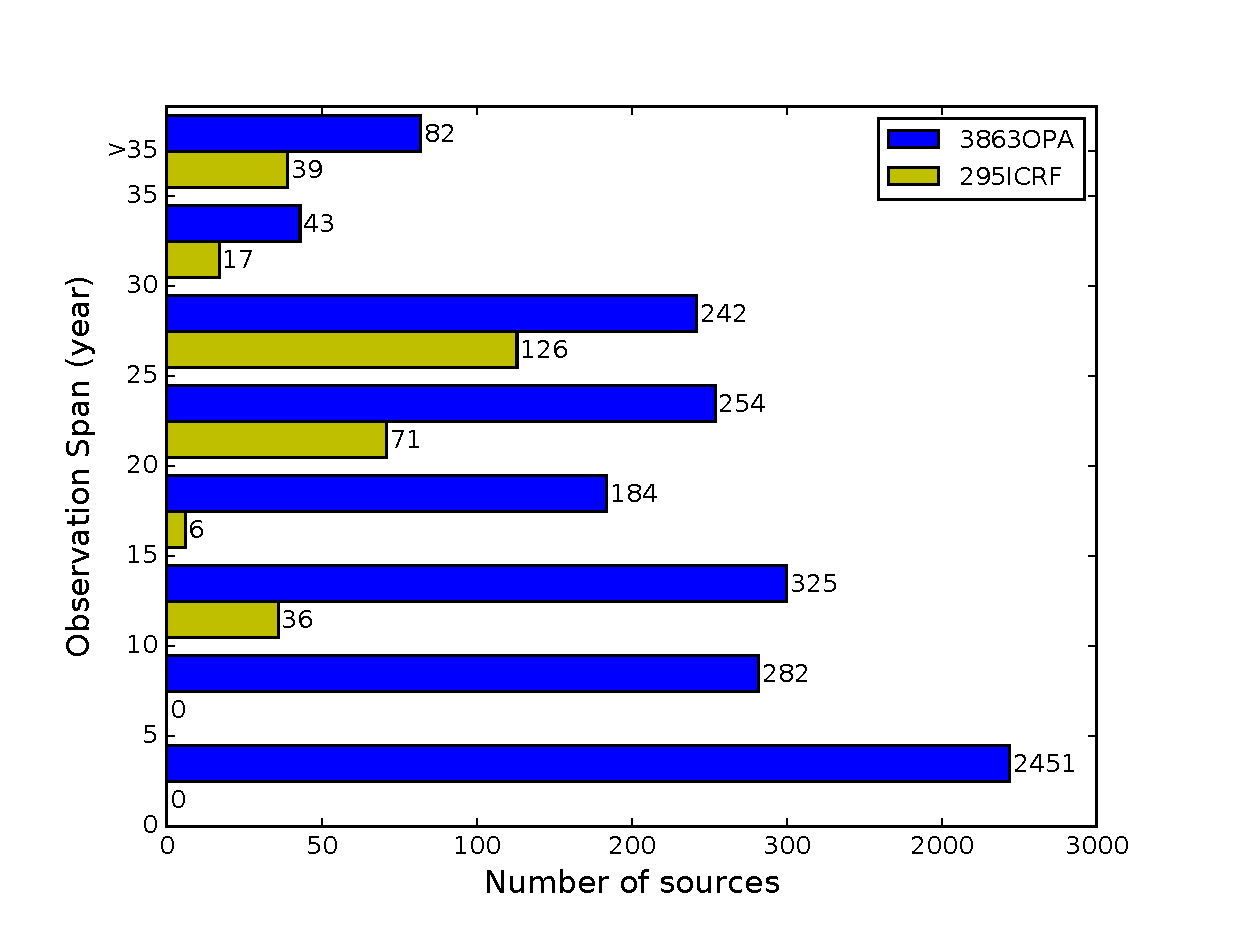
\includegraphics[width=0.45\hsize]{figures/Observation_span}}
   \subfigure[]{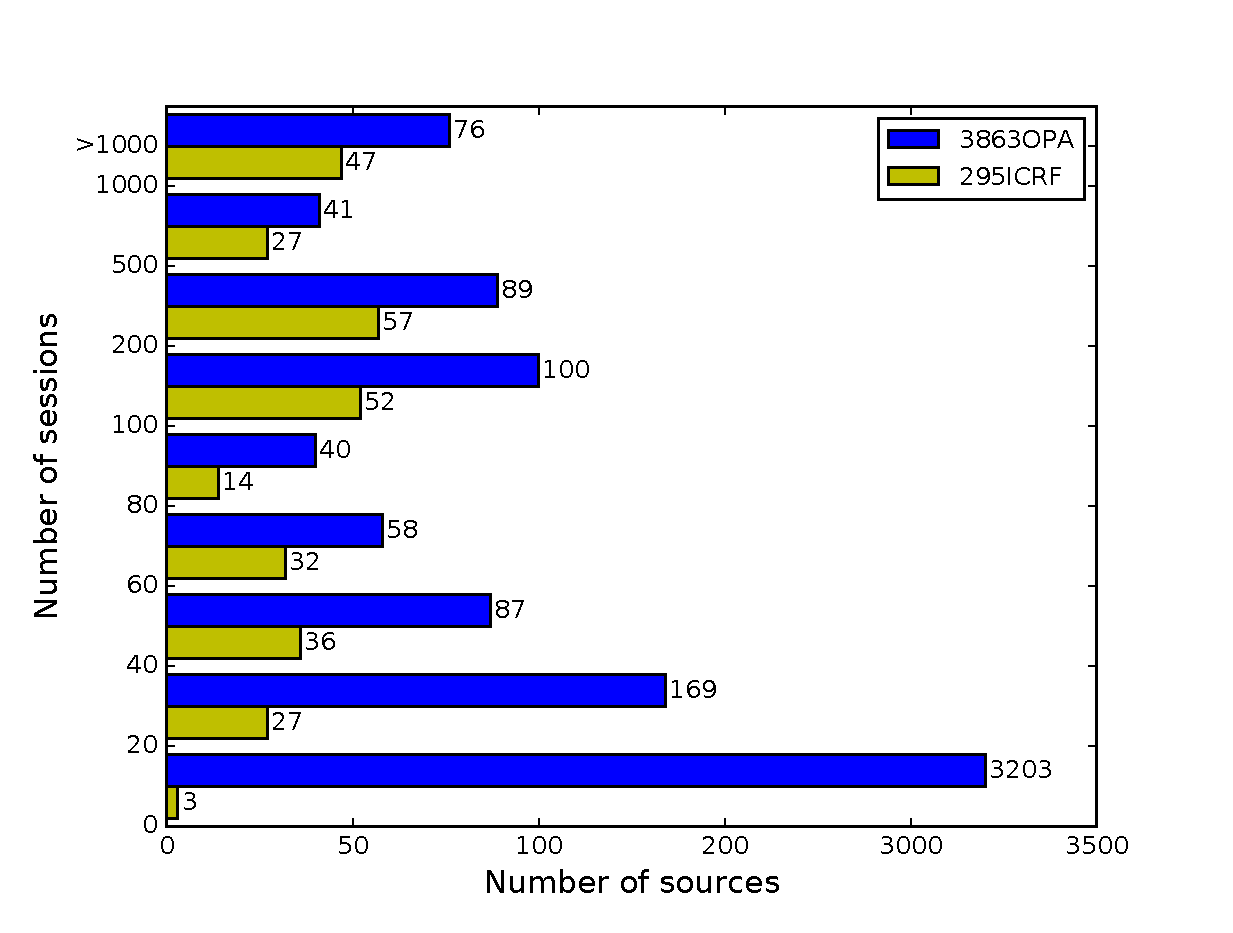
\includegraphics[width=0.45\hsize]{figures/Number_of_session}}
      \caption{Statical histograms of length of the observation span ($left$) and amount of the observational session for a individual source ($right$), displaying the observational histories of the 3826 sources. 
              }
         \label{Fig:Observation}
   \end{figure*}
%   \begin{figure}
%   \centering
%   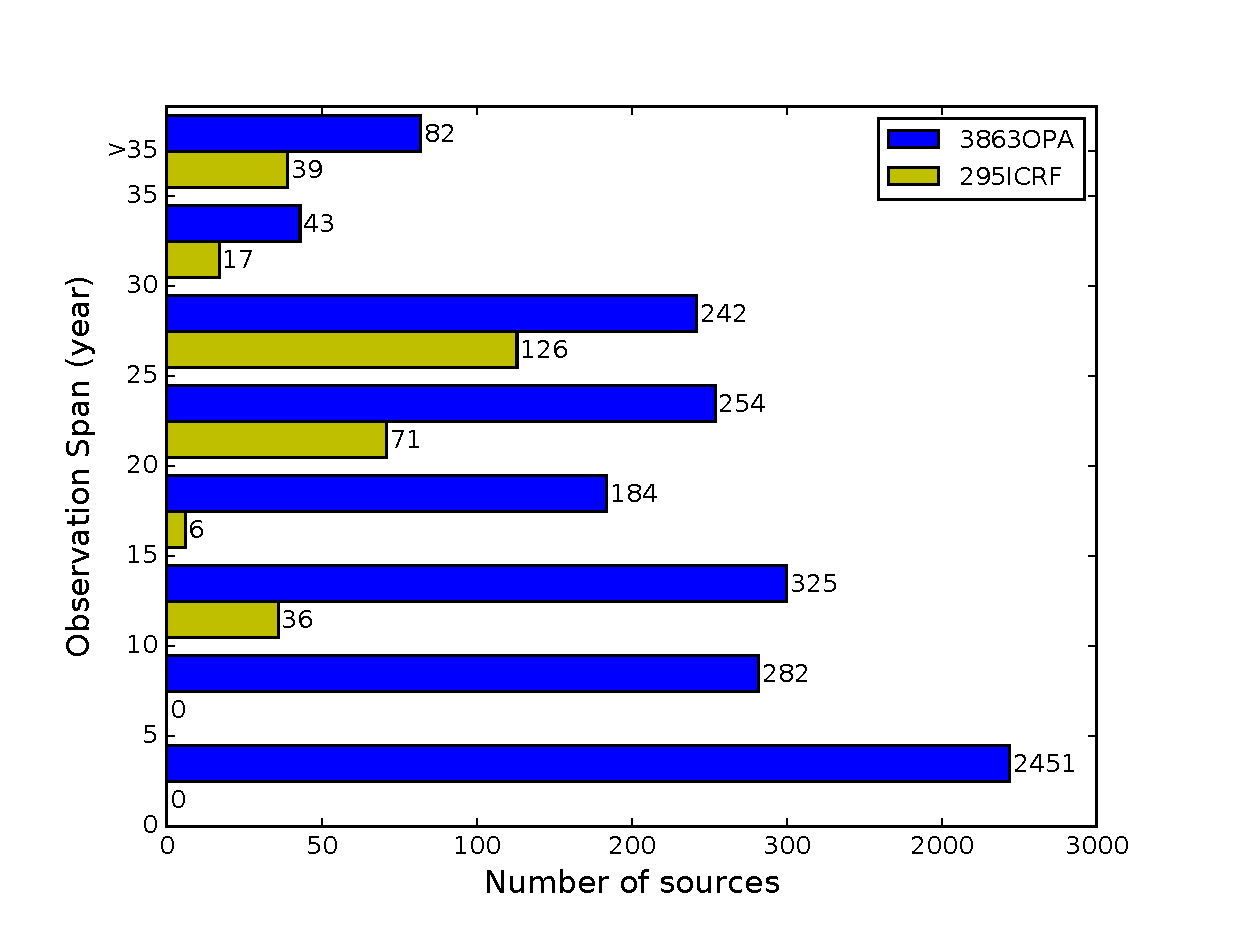
\includegraphics[width=0.5\hsize]{figures/Observation_span.eps}
%      \caption{
%      The length of observation history.
%              }
%         \label{Fig:ObsSpn}
%   \end{figure}
%
%   \begin{figure}
%   \centering
%   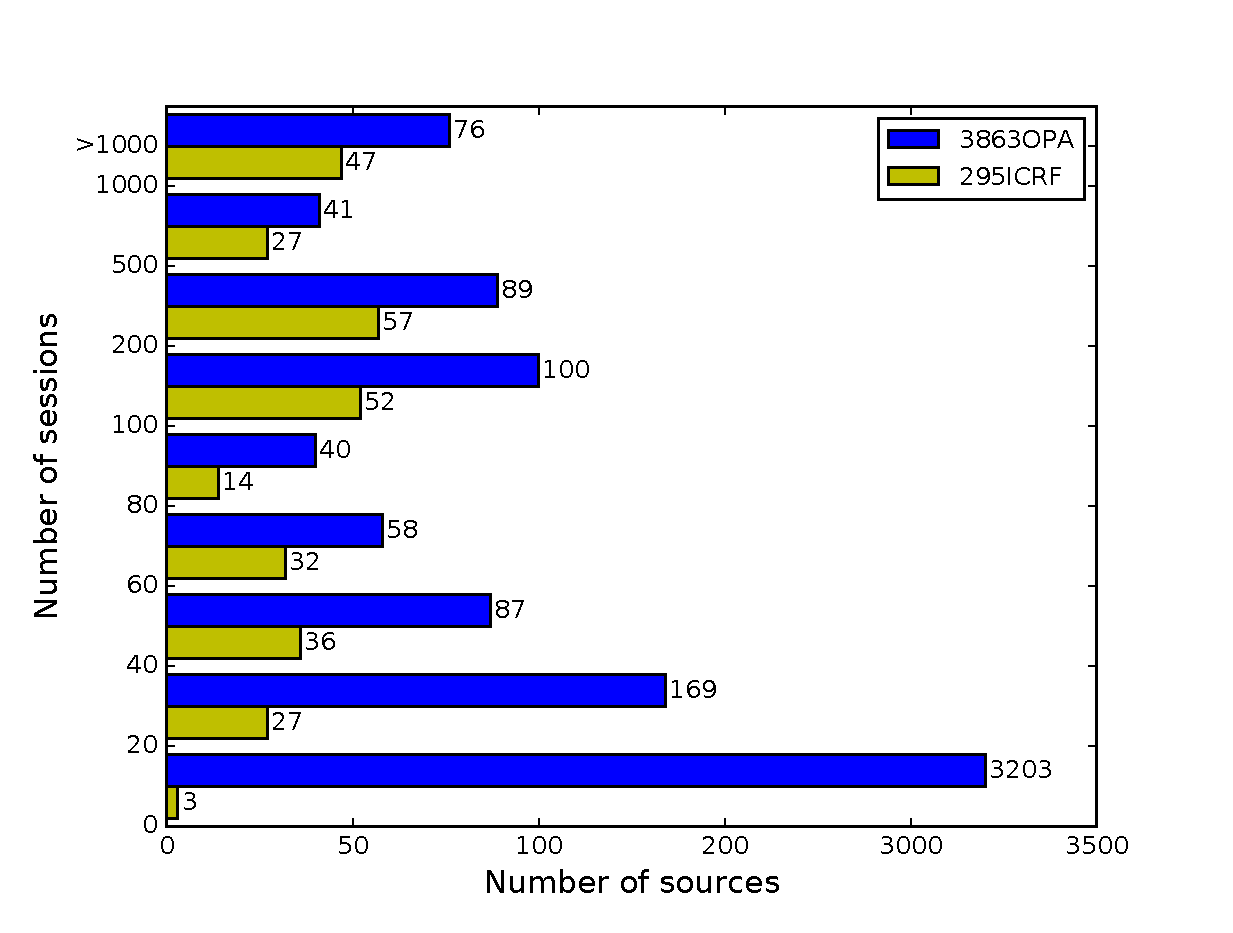
\includegraphics[width=0.5\hsize]{figures/Number_of_session.eps}
%      \caption{
%      Number of sessions in which a given source is observed. The bar above 1000 means that these sources are observed in more than 1000 sessions.
%              }
%         \label{Fig:NumSes}
%   \end{figure}
   
\begin{figure}
   \centering
   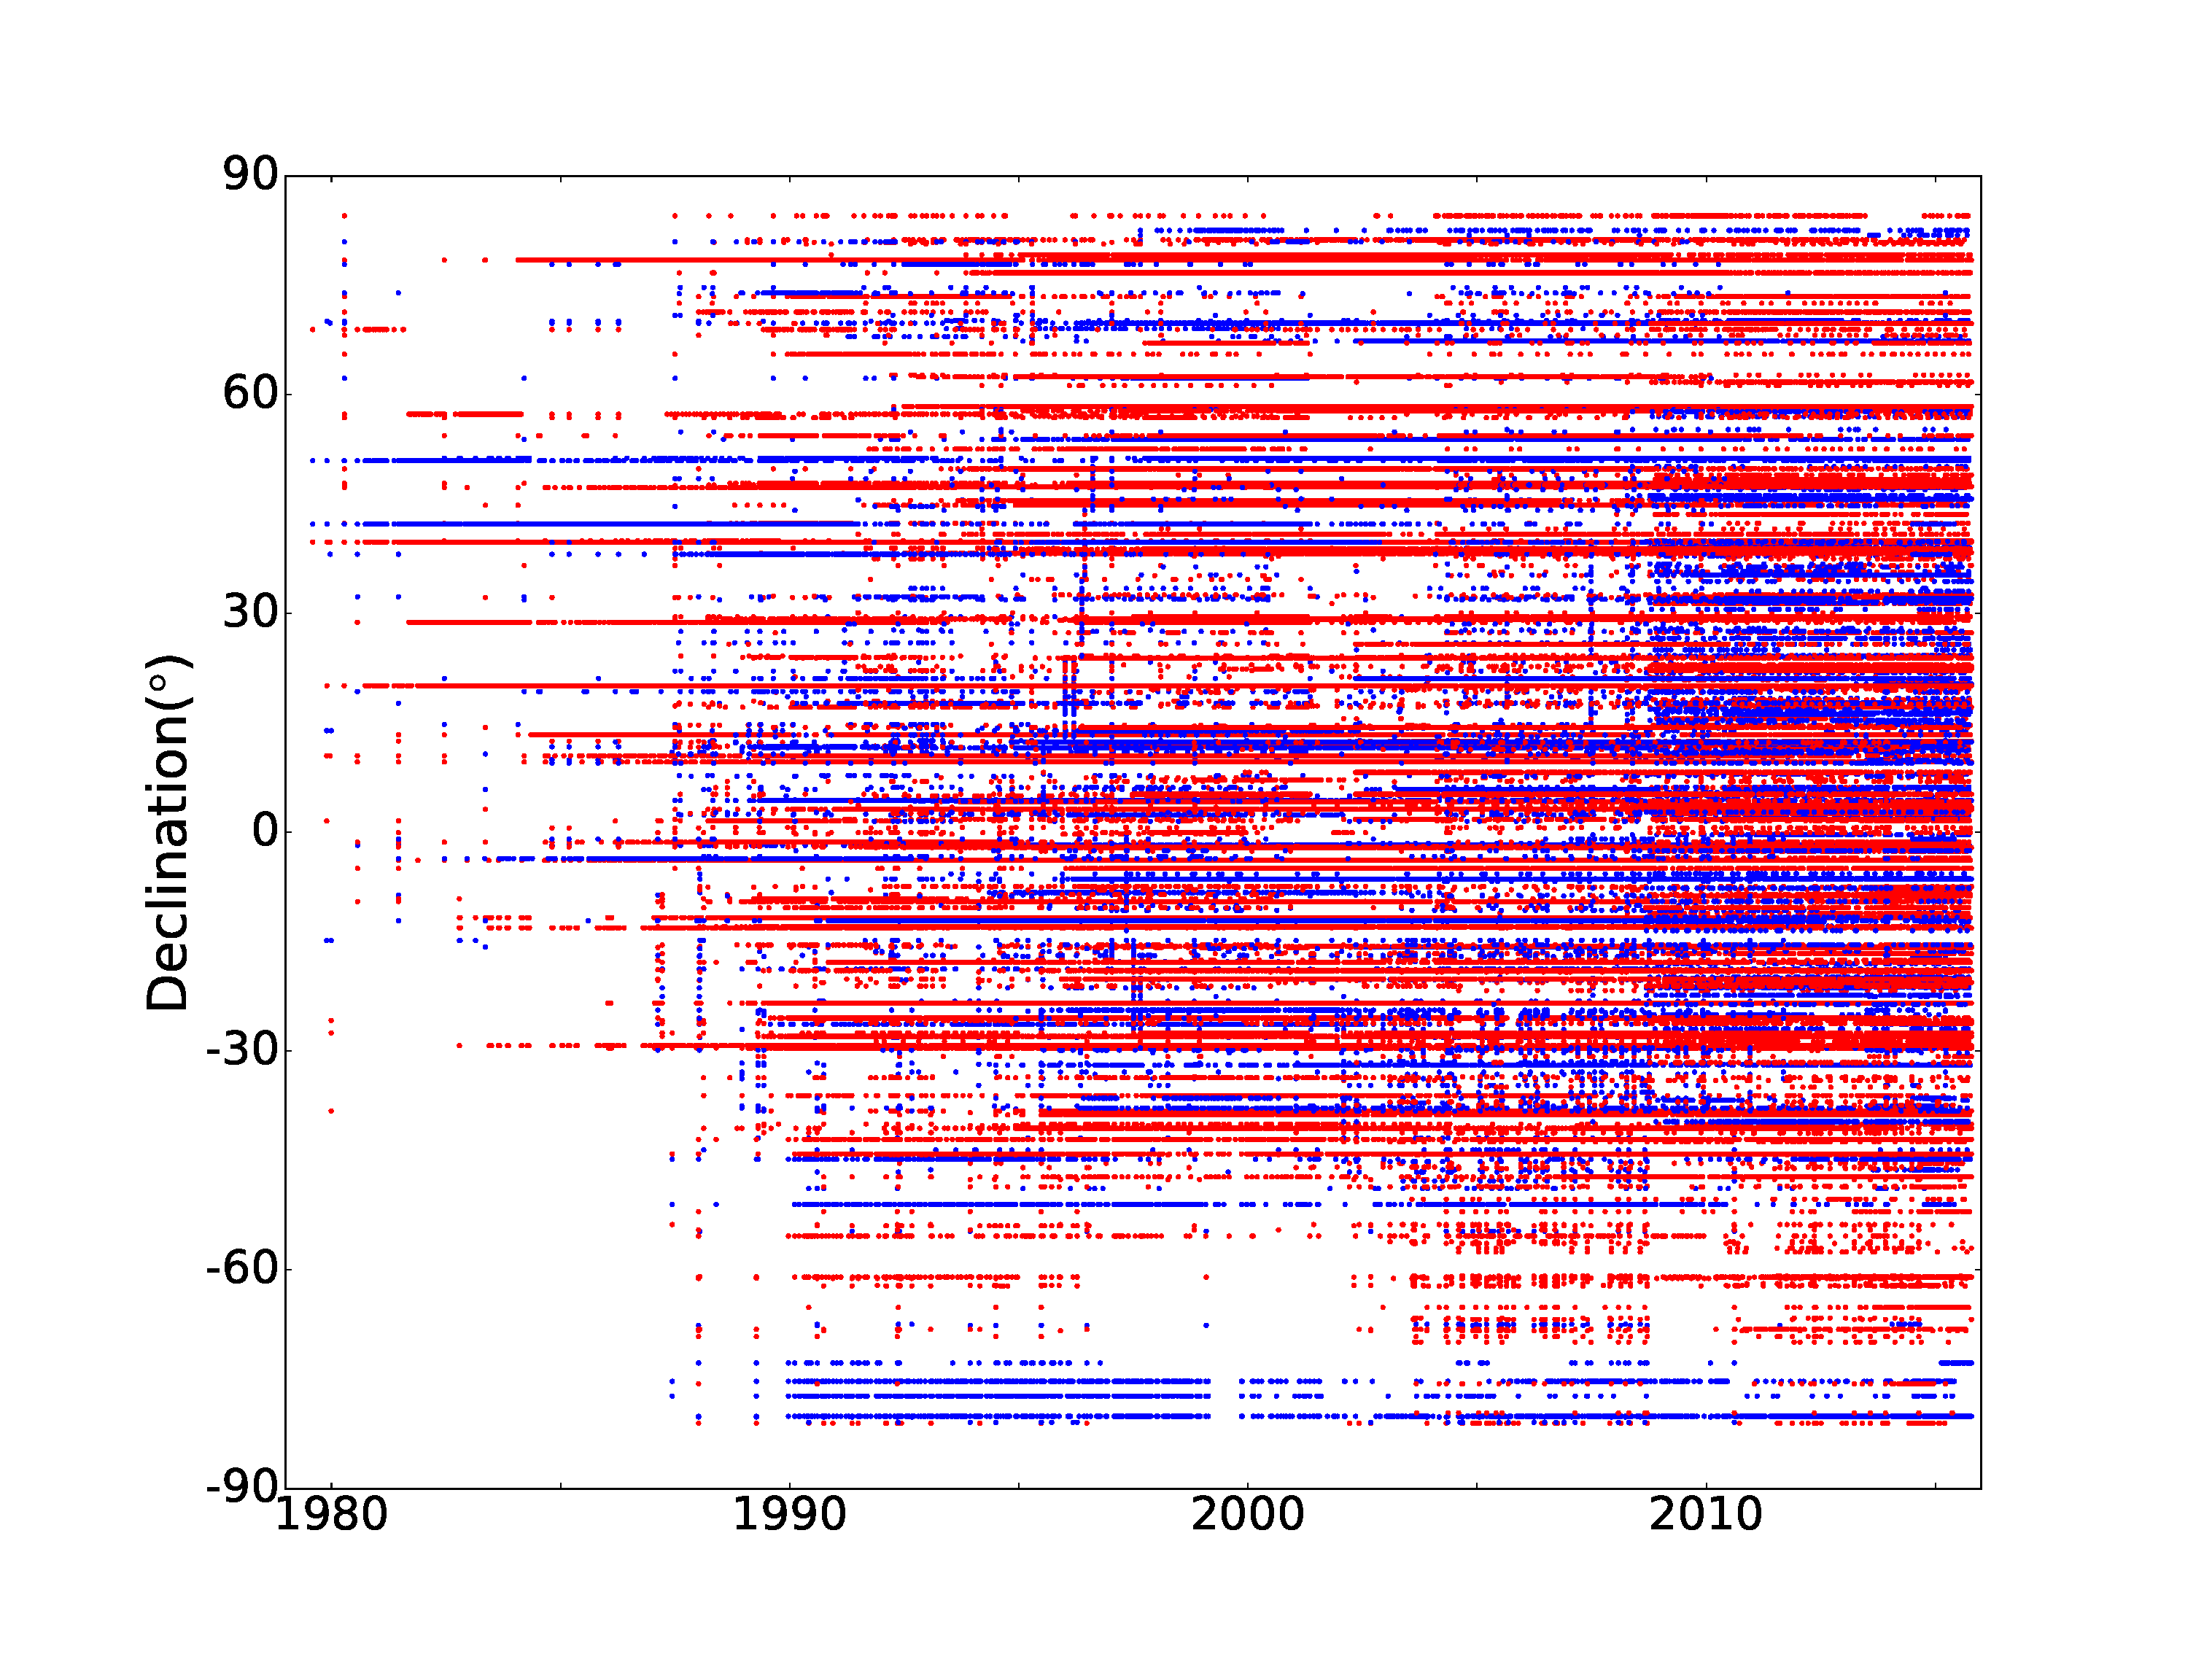
\includegraphics[width=\hsize]{figures/Observation_history.eps}
%	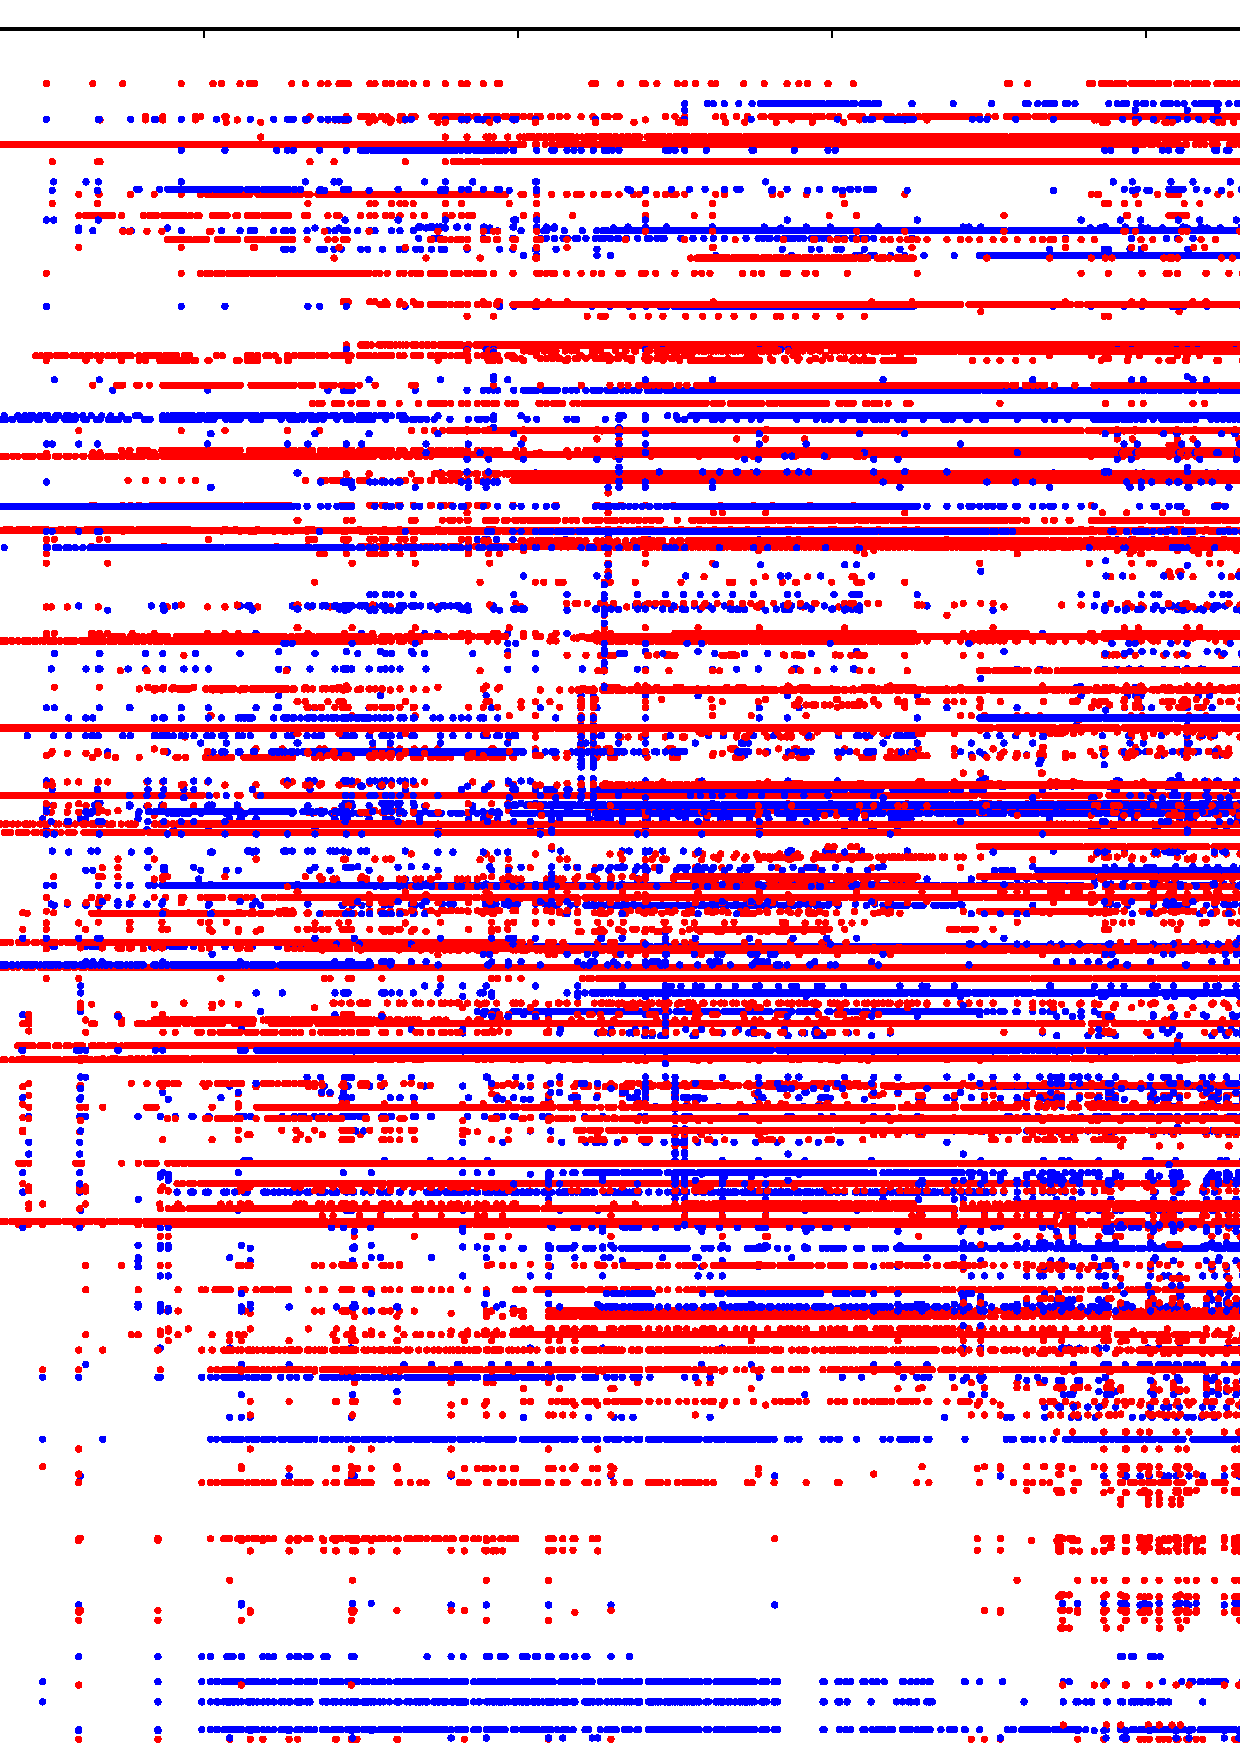
\includegraphics[width=\hsize ,bb=0 0 1440 1080]{figures/Observation_history.PNG} 1
      \caption{
      Observation history of 613 sources, including 291 ICRF2 defining sources ($red$) and 322 non-defining sources ($blue$).
              }
         \label{Fig:ObsHis}
\end{figure}

%-----------------------------------------------------------------
\section{Sources Selection}\label{sect:select}
Although the radio sources are assumed to have no proper motion because of their extremely far distances, the time series of coordinates will show some variability, due to i.e., an immediate rejection of jet or the extend structure, affecting the stability of the celestial frame based on them. The variability can be investigated by statistical estimators, i.e., the goodness of fit considered as an indictor sensitive to random errors. Three estimators are used in this paper: the weighted standard deviation referred to the mean (weigthed root mean square), the weighted Allan deviation and the linear drift (slope) of both $\alpha\cos\delta$ and $\delta$ coordinates. The standard deviation decribles the scatters of the coordinates while the Allan deviation investigates the stochastic properties of coordinates time series, sensitive to abrupt changes of coordinates. And the linear drift estimation is based on an underlying physical assumption, and considered as reliable since time series of these candidates have enough many points. In this work, the weighted standard deviation and the weighted Allan deviation are estimated to rule out sources with significantly noisy time series while the normalized linear drift (the ratio of linear drift to its uncertainty) is used as an indicator of positional stability, according to which the sources are ranked from most stable to less in the next precedure.

Annual average points are constructed by taking the weighted mean of all data contained in an one-year interval over 1980.0-2016.0 for determination of the Allan deviation. However, few sources have observational histories dense enough for the Allan deviation test. An extension of the Allan deviation proposed by \cite{Malkin2008} (labelled as "WADEV" in that paper) is used. 

Fig. \ref{Fig:Dev} presents the distribution of the weighted standard deviation and the weighted Allan deviation. The result is much larger compared to that of \cite{F-V2003}. The possible reason is that the entire time series are used here while post-1990.0 time series were used in that work. Then sources with the weighted standard deviation or the weighted Allan deviation of both coordinates larger than $10mas$ are excluded, and 499 sources are kept.

The linear drifts are obtained using the weighted least squares estimation but there is a difference. Consider that the formal error is an accumulative effect during the data reduction and may not be the real observational error, average weight over a observationan span is used. The time series are devided into three observation spans: 1979.0$\sim$1990.0; 1990.0$\sim$2009.0; 2009.0$\sim$2016.0, on the assumption that each observation span corresponds to different observational accuracies. And the average weight is used as weight of session points within the corresponding observation span. The normal equation of estimation of $\alpha\cos\delta$ coordinate is  given by (\ref{eq:normal}) and the one for $\delta$ coordinate is similar. 

\begin{equation}
\label{eq:normal}
\left(
	\begin{array}{c}
	\mu _{\alpha ^{*}} \\
	\alpha ^{*}_0
	\end{array}
\right)
	= \sum _{i=1}^3
\left(
	\begin{array}{cc}
	\sum\limits _j \dfrac{(\Delta t_{ij} )^2}{\sigma ^2_{ij}} & \sum\limits_j \dfrac{(\Delta t_{ij})}{\sigma ^2_{ij}} \\
	\sum\limits_j \dfrac{(\Delta t_{ij})}{\sigma ^2_{ij}}   & \sum\limits_j \dfrac{1}{\sigma ^2_{ij}}
	\end{array}
\right) ^{-1}
\left(
	\begin{array}{c}
	\sum\limits_j \dfrac{(\Delta t_{ij})\alpha ^{*}_{ij}}{\sigma ^2_{ij}} \\
	\sum\limits_j \dfrac{\alpha ^{*}_{ij}}{\sigma _{ij} ^2}  
	\end{array}
\right)
\end{equation} 

where $i=1, 2, 3$ represent the three observation spans respectively, and $\Delta t_{ij}$ is the difference refered to 2000.0. Silimar to the marker used in other papers, $\mu _{\alpha ^*} = \mu _{\alpha}\cos\delta$. Then the  linear drift $\mu = \sqrt{ \mu_{\alpha ^*}^2 + \mu ^2_\delta}$. 

Fig. \ref{Fig:Liner_drift_3} shows the linear drift of the three subsets, in which some sources are found to have the linear drift larger than 0.5 mas/yr (marked in red arrows). But it may be arbitrary to consider these sources as unstable, for  the corresponding uncertainties of the linear drift may be large too. A sources with a large linear drift and small corresponding uncertainty is more possible to be unstable \citep{Lambert2009}. For this reason, sources are ranked from the most stable to less according to their normalized linear drift. This rank list will be referred as "OverallRank list" in the following sections. However, because of the less sources in the southern hemisphere, small number will enter the defining sources list according to OverRank list, causing the celestial frame uniform. To loose the threshold for sources with low declination, the ICRF2 work introduces a method in which sources are binned into 6 intervals of declination by four nodes so that each interval has approximately the same number of sources. In each interval, sources are given a rank index normalized 100, and ranked. Here another way is adopted. The sphere are divided into 4 partitions with the equal spherical area, and the corresponding nodes of the declination are $-30^{\circ}$, $0^{\circ}$ and $30^{\circ}$. The number of sources located in partitions are 77, 126, 161 and 135 respectively. In each partition, similarly, sources are ranked according to the normalized linear drift. In the final rank list, the sources with smaller rank order are ranked more priori, while the ranking priorities of sources with same rank order in different partitions are based on their normalized linear drift. Using this rank strategy, a rank list referred as "PartitionRank list" is established. In the next part, we will determine the subsets of stable sources according these two rank list.

\begin{figure}
   \centering
   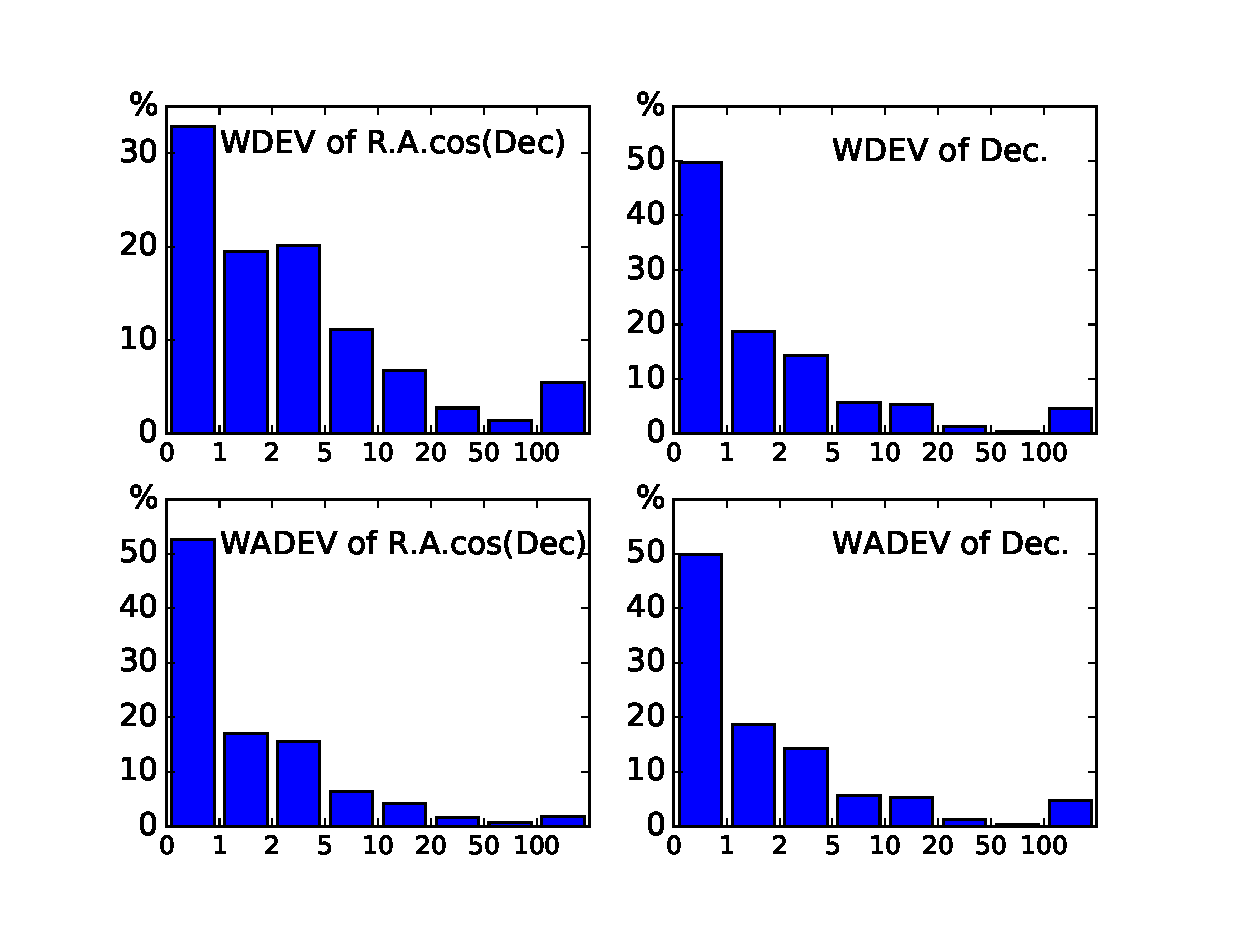
\includegraphics[width=\hsize]{figures/DEV_plot.eps}
      \caption{
      The statistical histograms of the weighted standard deviation (WDEV) and the weighted Allan deviation (WADEV) for $\alpha\cos\delta$ ($left$) and $\delta$ ($right$) coordinates. The units are mas.
              }
         \label{Fig:Dev}
\end{figure}

\begin{figure*}
   \centering
   \subfigure[212 ICRF]{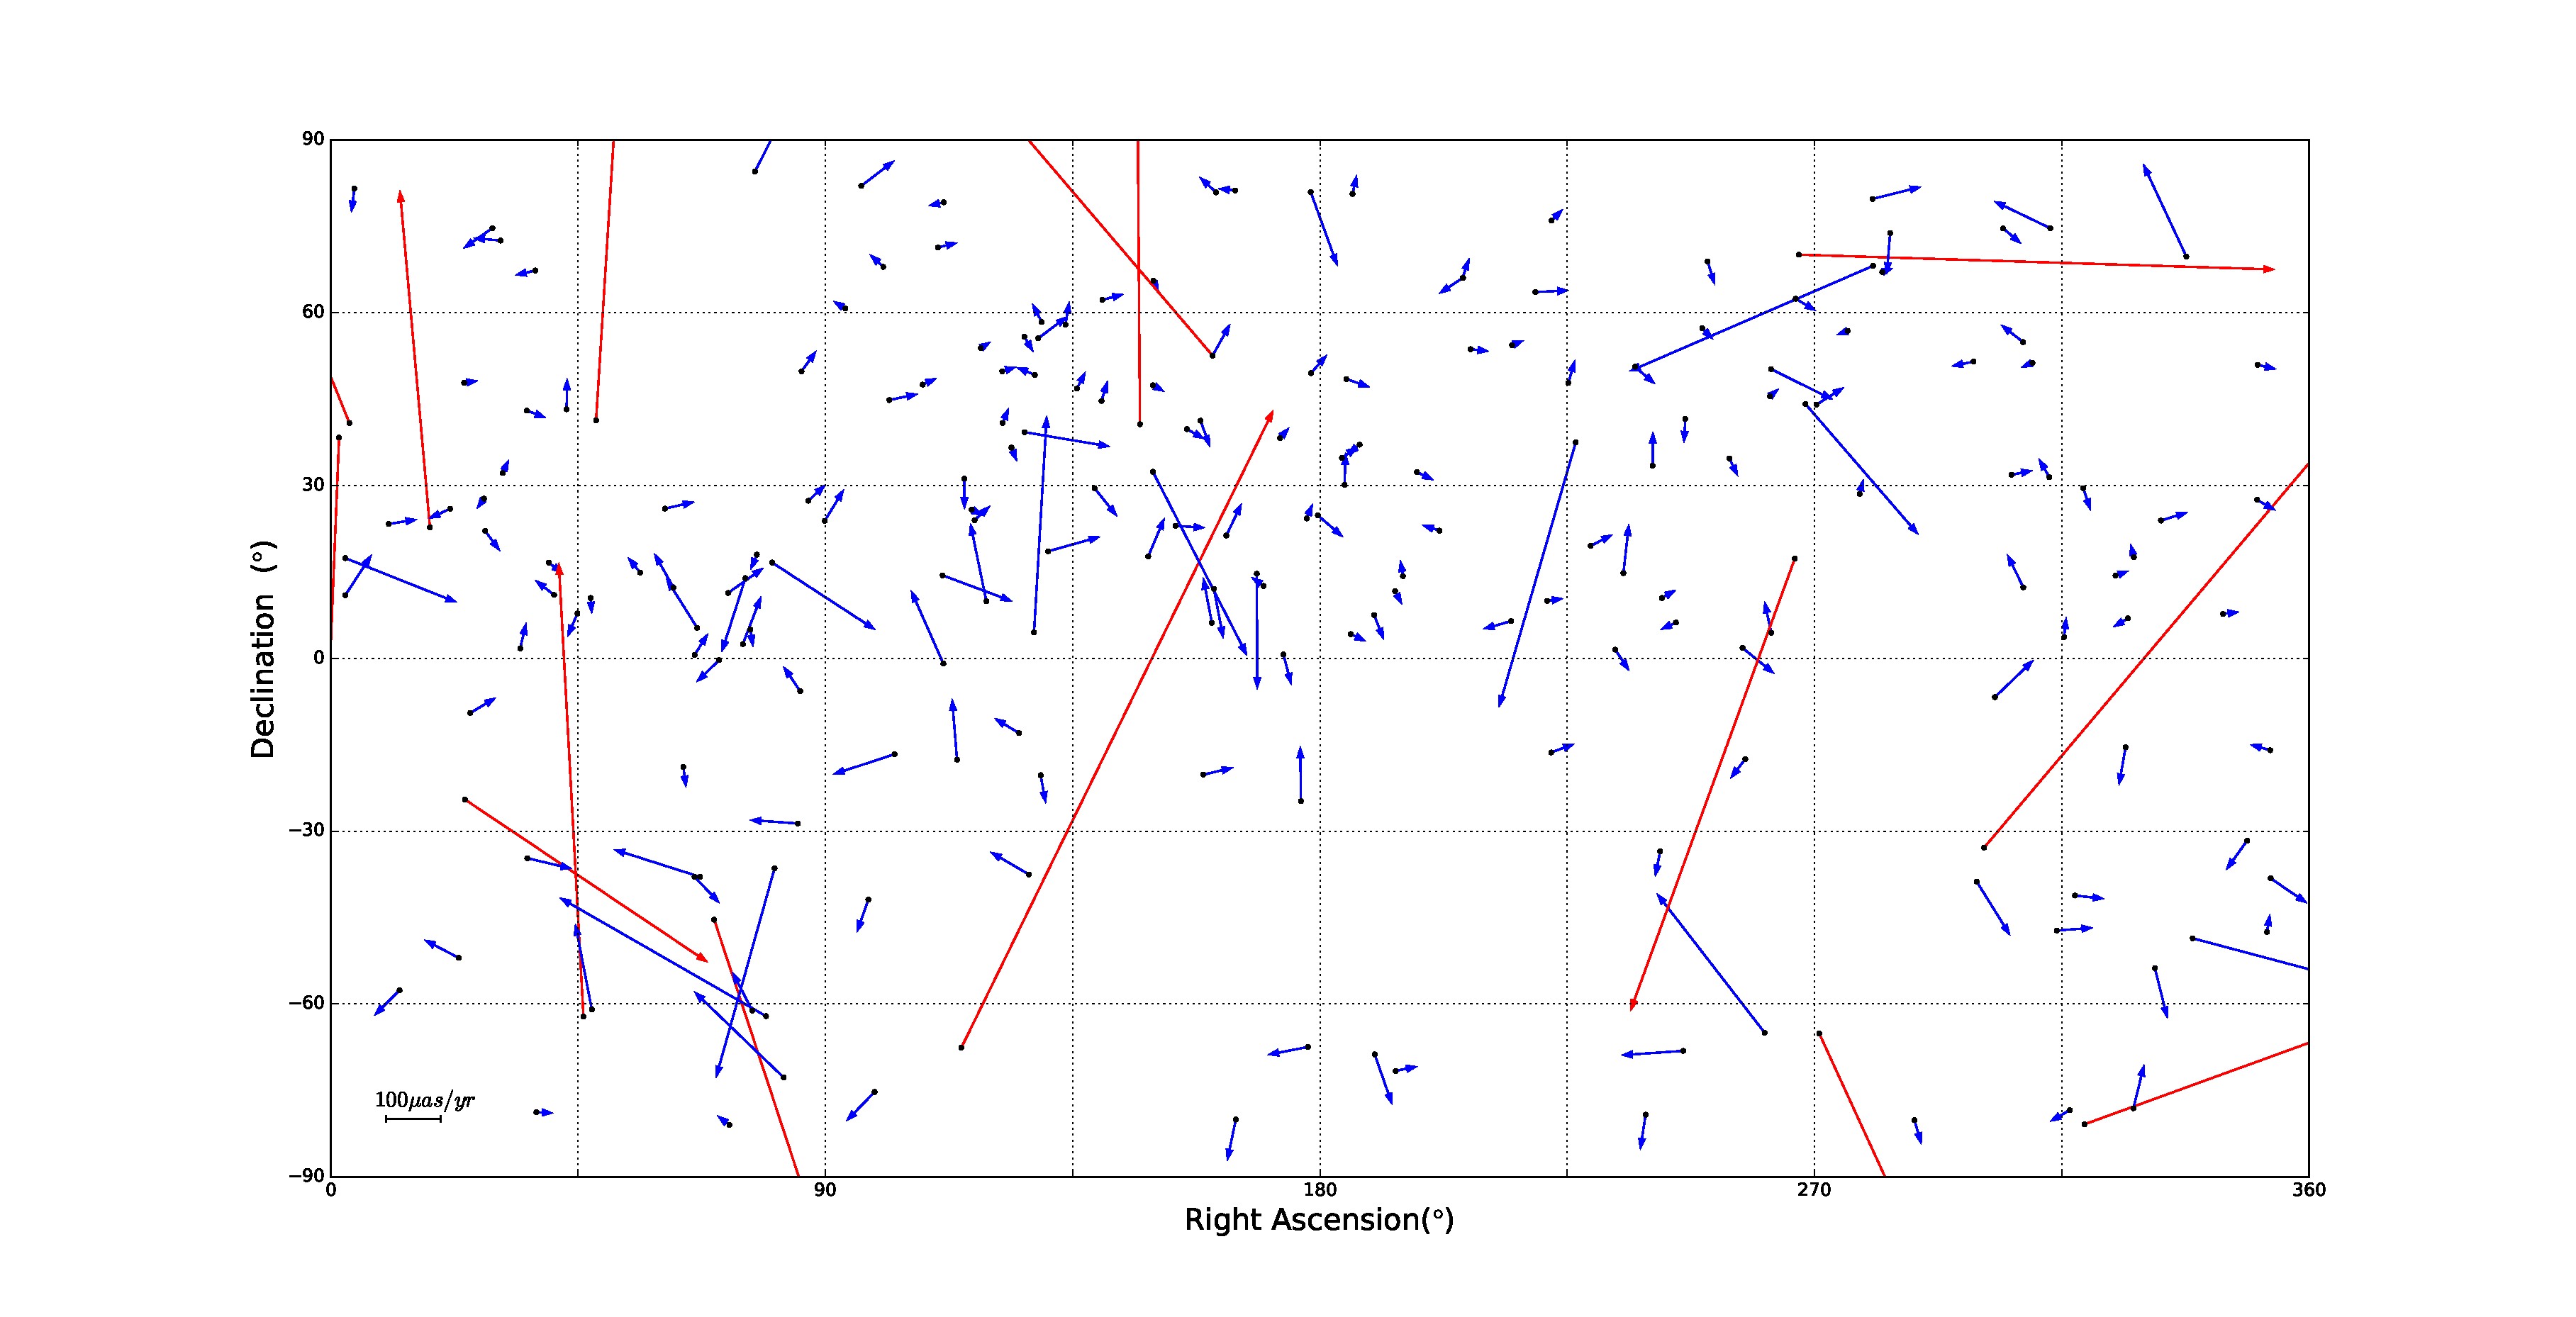
\includegraphics[width=0.5\hsize]{figures/Linear_drift_icrf1.eps}}
   \subfigure[295 ICRF2]{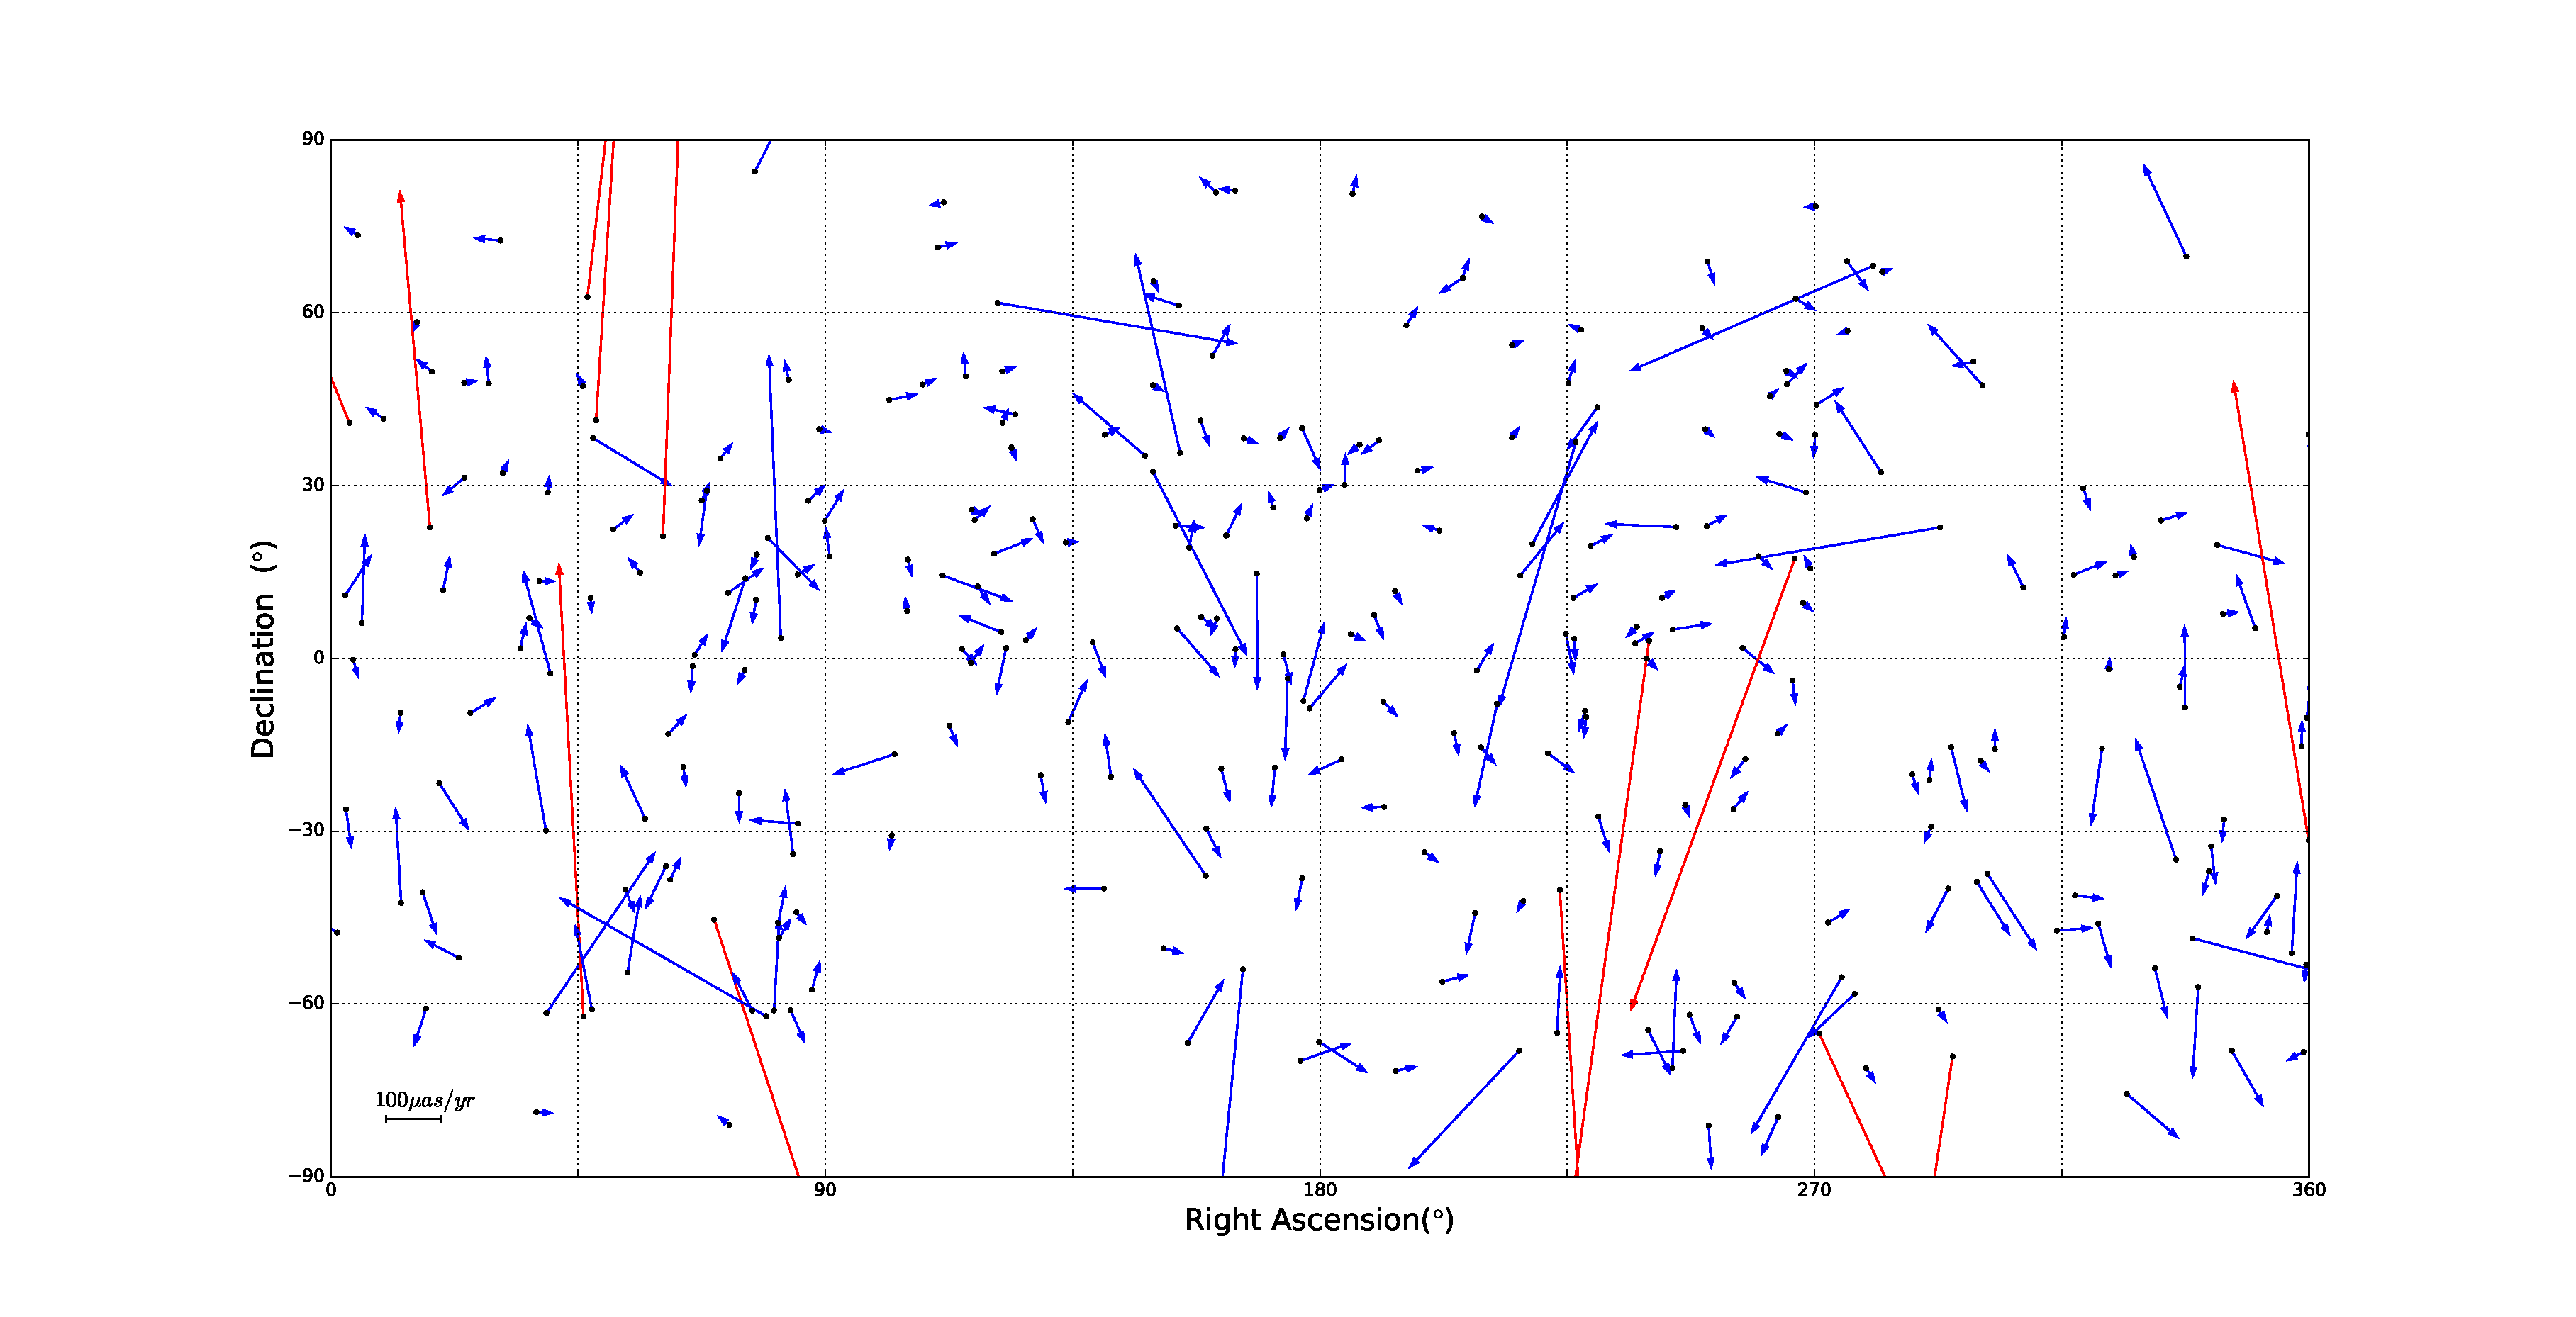
\includegraphics[width=0.5\hsize]{figures/Linear_drift_icrf2.eps}}
   \subfigure[247 MFV]{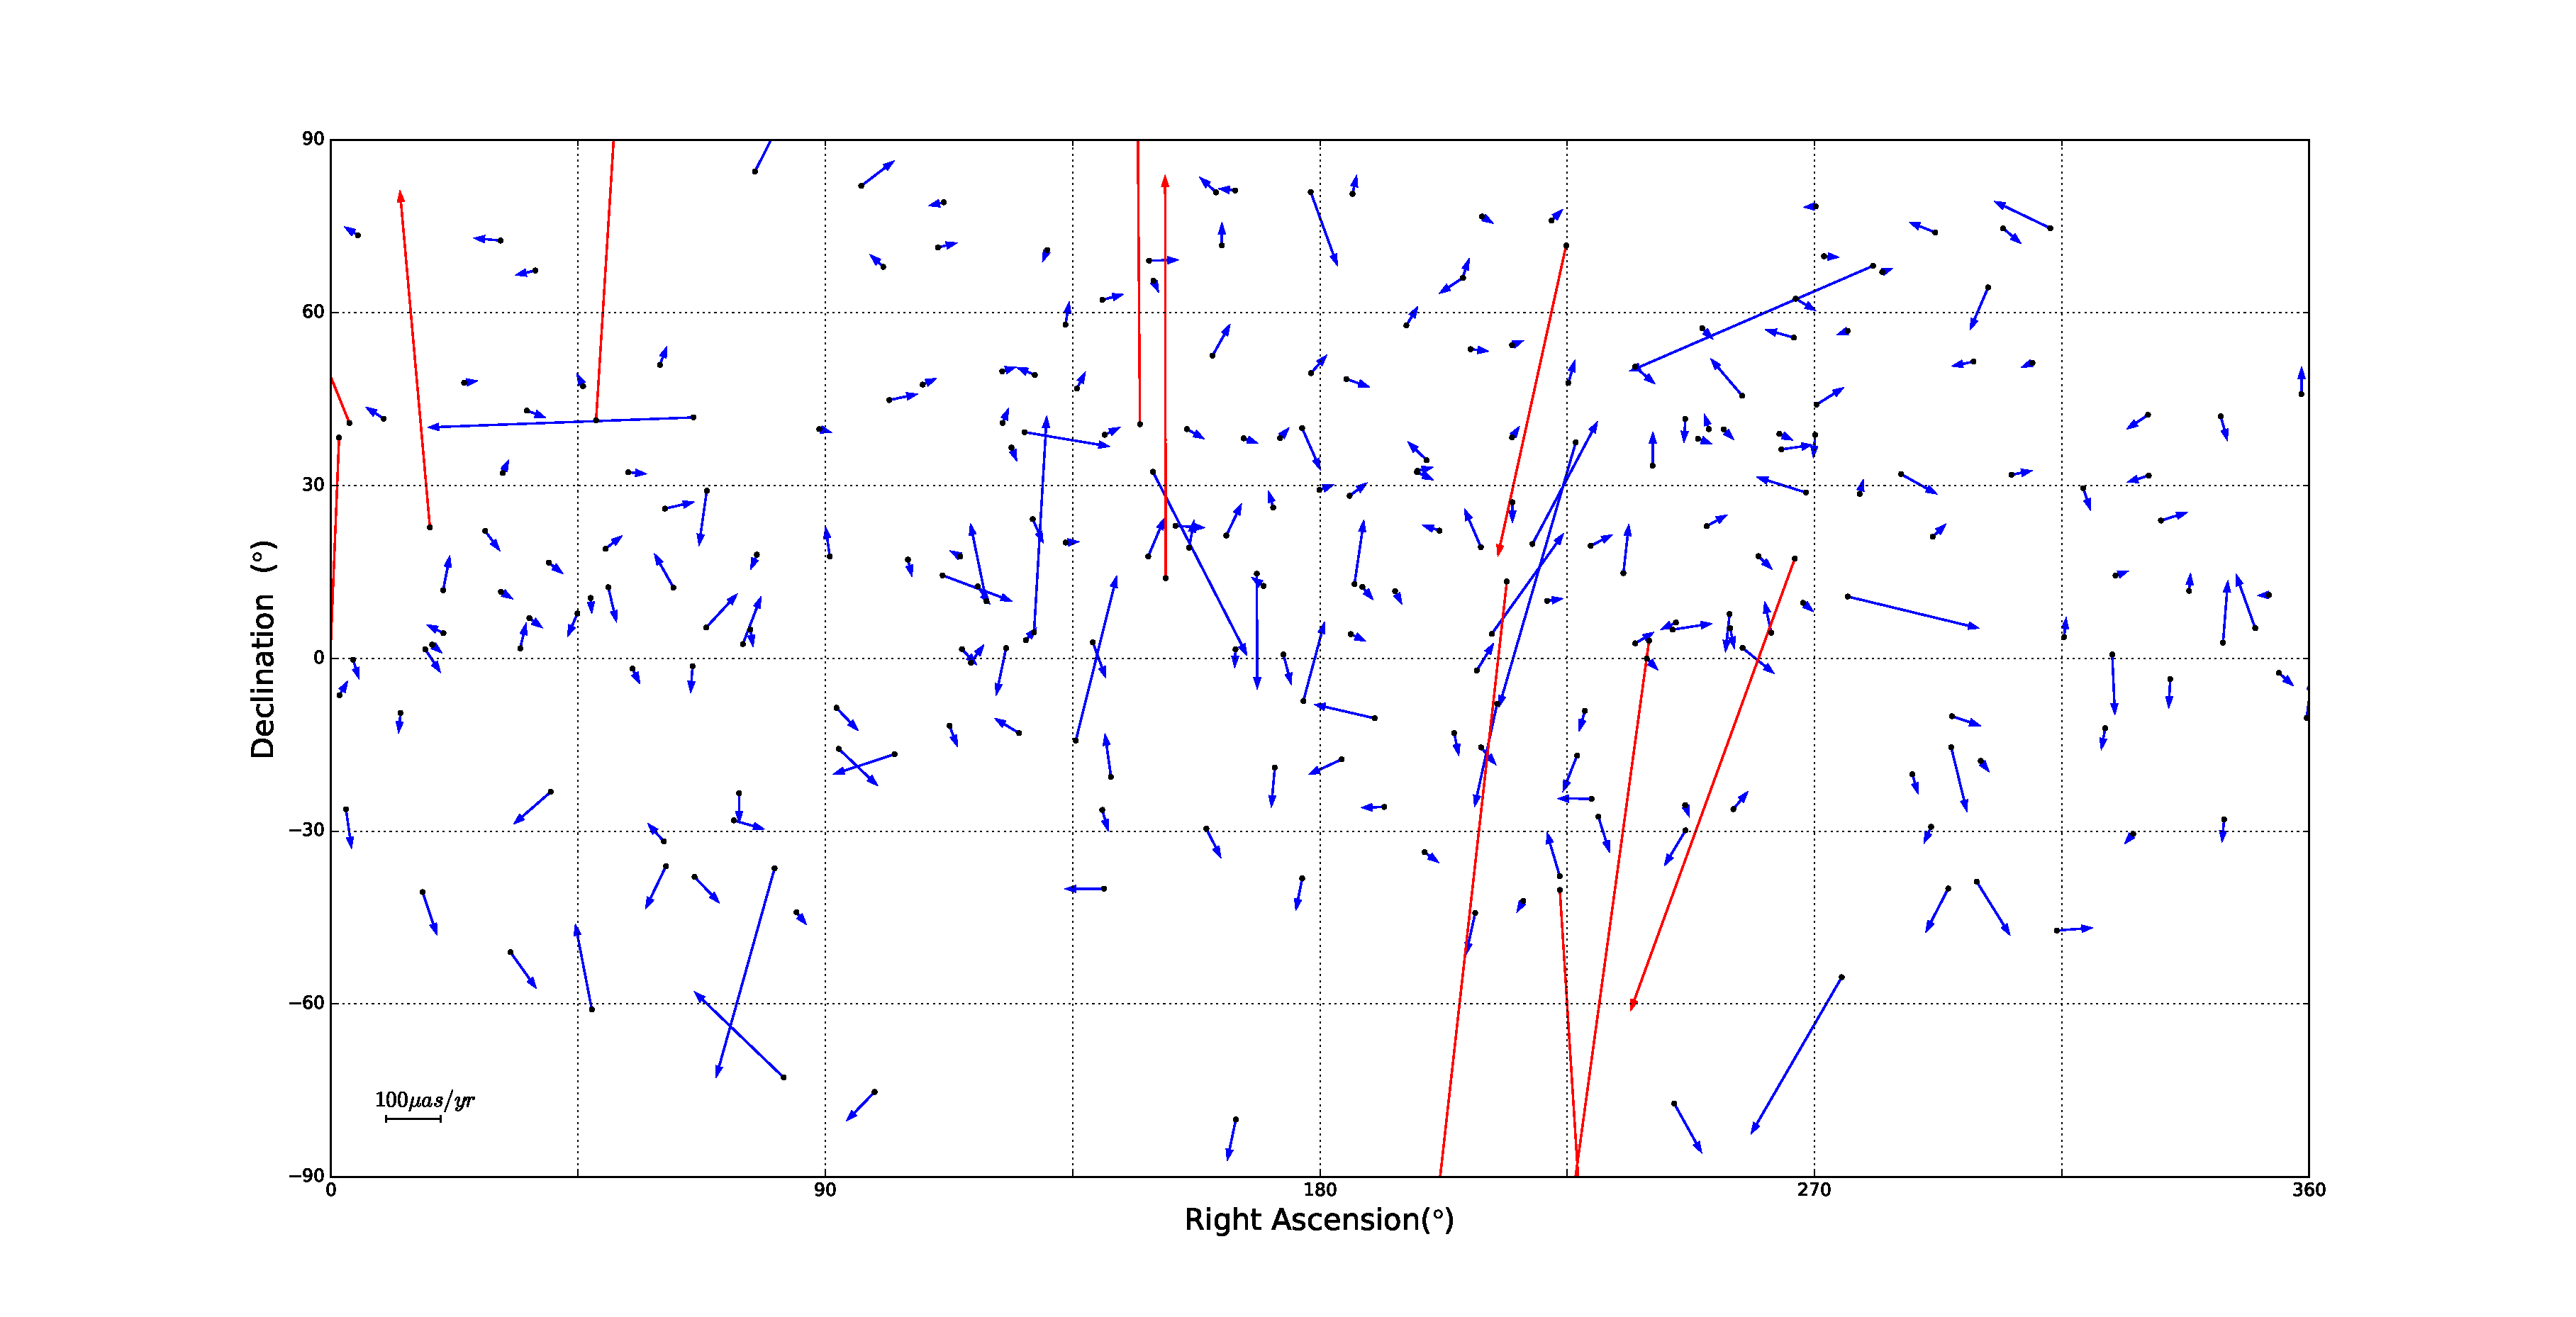
\includegraphics[width=0.5\hsize]{figures/Linear_drift_mfv247.eps}}
      \caption{
      Linear drift of three sets of sources selected in previous works. The red arrows indicate the corresponding values are larger than 500 $\mu as\cdot yr^{-1}$.
      %: 212 ICRF defining($top$), 295 ICRF2 defining($middle$) and 247 MFV($bottom$).
              }
         \label{Fig:Liner_drift_3}
   \end{figure*}
%
\subsection{Considerations on the axial stability}
The stability of reference frame axes is usually 
The stability of reference frame can be assessed by fitting the one-order spherical harmonics coefficients of rotation to the linear drift, in which the equations are given below.
%% (citation.):
\begin{eqnarray}
      \mu_{\alpha}\cos\delta & = 
                                & +r_1\cos\alpha\sin\delta +r_2\sin\alpha\sin\delta -r_3\cos\delta \\
      \mu_{\delta}           & = 
      						    & -r_1\sin\alpha + r_2\cos\alpha,
   \end{eqnarray}
   where ($r_1$,$r_2$,$r_3$) is the three coordinate part of global rotation.
The total rotation of reference frame can be given by $r = \sqrt{r_i^2 }$. Fig. \ref{Fig:rot_num} shows $r_1, r_2, r_3$ and r evolve with the number of sources. It is obviously seen from the overall trend that as the number increases, more sources with large $\mu$ are included in, causing larger axial rotations for both ranks. But there are some eclipses and horns. And for r, a eclipse appears for rank1 while a horn for rank2 when number is around 200. 

When considering the influence of one-order glide vector in the spherical harmonics fitting, the equations are shown in the below:
%citation
\begin{eqnarray}
      \mu_{\alpha}\cos\delta & = 
                             & -g_1\sin\alpha + g_2\cos\alpha                    \nonumber                                             \\
                         &   & +r_1\cos\alpha\sin\delta +r_2\sin\alpha\sin\delta -r_3\cos\delta                \\
      \mu_{\delta}           & = 
                             & -g_1\cos\alpha\sin\delta -g_2\sin\alpha\sin\delta +g_3\cos\delta  \nonumber     	\\					                     &   & -r_1\sin\alpha + r_2\cos\alpha,
   \end{eqnarray}
   where ($g_1$,$g_2$,$g_3$) is the three coordinate part of glide vector.
%
Fig. \ref{Fig:Rot_gli} displays the result, which shows that with more than 250 sources, the rotation part is close to the one in Fig. \ref{Fig:rot_num}, while glide part shows no pattern.

\begin{figure}
   \centering
   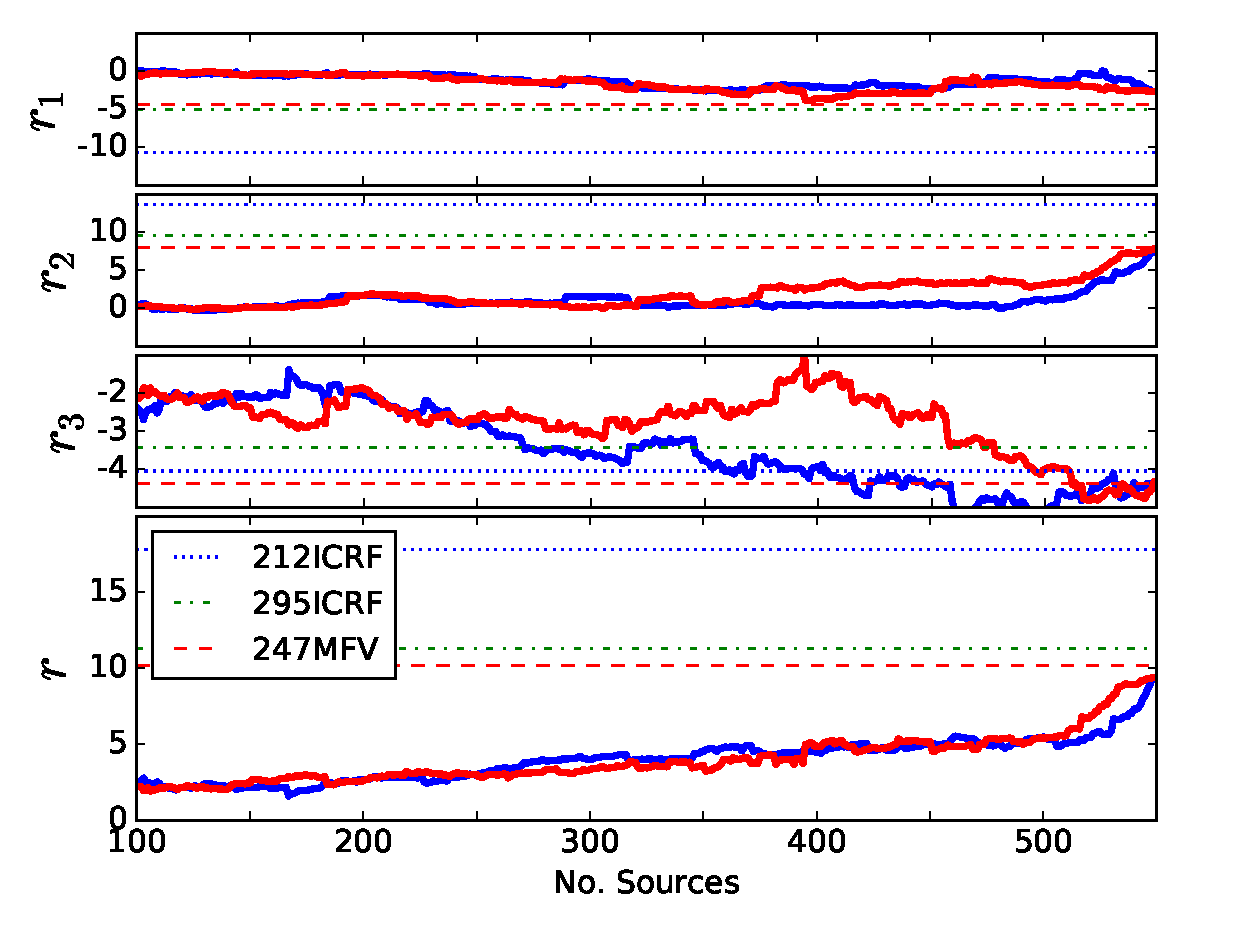
\includegraphics[width=\hsize]{figures/Rot_num.eps}
%   \includegraphics[width=\hsize]{figures/OARank_rot.eps}
      \caption{
      The fitting results of considering rotation vector only. The blue and red line are corresponding result of rank1 and rank2 respectively.
              }
         \label{Fig:rot_num}
\end{figure}

	\begin{figure}
   \centering
   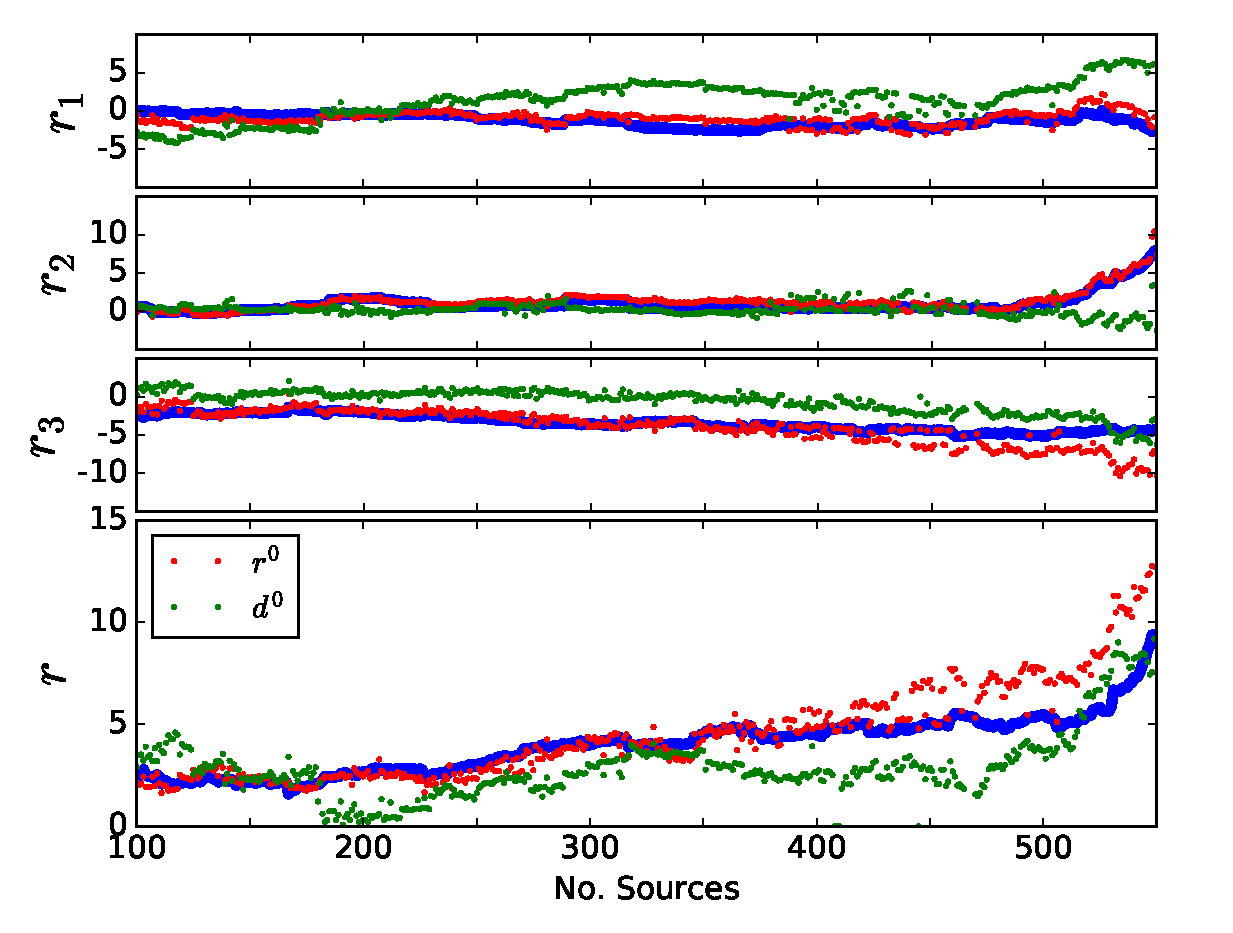
\includegraphics[width=\hsize]{figures/Rot_Gli.eps}
      \caption{
      The fitting results of considering rotation and glide vector. The blue line is the result shown in Fig . The red and green piont are  corresponding part of rotation and glide respectively. The rank way is rank1.
              }
         \label{Fig:Rot_gli}
   \end{figure}

\subsection{Considerations On the sky distribution}
How uniform the sources distribution on the sphere sky is, is another aspect that need to be taken into consideration. Here a simulation is adopted to test the different set of sources. First all sources are assumed to have a proper motion towards a center, and a dipole vector filed ($\mu_{\alpha s}, \mu_{\delta s}$) is given by equation shown below. 
\begin{eqnarray}
      \mu_{\alpha s}\cos\delta & = 
                             & -d_1\sin\alpha + d_2\cos\alpha                                                                 \\
      \mu_{\delta s}           & = 
                             & -d_1\cos\alpha\sin\delta -d_2\sin\alpha\sin\delta +d_3\cos\delta,
   \end{eqnarray}
where $d_1 = A\cos\alpha_0\cos\delta_0$, $d_2 = A\sin\alpha_0\cos\delta_0$, and $d_3 = A\sin\delta_0$ are these components of acceleration vector, and A is a constant. Here $A = 5 \mu as\cdot yr^{-1}$, $\alpha_0 = 0^{\circ}$, and $\delta_0 = 90^{\circ}$.  Then one-order spherical harmonics of rotation is fitting the vector filed ($\mu_{\alpha s}, \mu_{\delta s}$), using the equations similarity to Eq
%citation
\begin{eqnarray}
      \mu_{\alpha s}\cos\delta & = 
                                & +\omega_1\cos\alpha\sin\delta +\omega_2\sin\alpha\sin\delta -\omega_3\cos\delta \\
      \mu_{\delta s}           & = 
      						    & +\omega_1\sin\alpha - \omega_2\cos\alpha,
   \end{eqnarray}
The total rotation $\omega$ is given by $\omega = \sqrt{\omega_i^2 }$
This approach was adopted in
%J—C,Liu  
, which gives a conclusion that for a set of sources with more uniform sky distribution $\omega$ is smaller. For a set of sources that have s ideal uniform sky distribution, $\omega = 0$. The result of simulation is shown by Fig. \ref{Fig:sim}, from which $\omega$ decreases where the number of sources increase as first, then has slight ups and downs.
And a close trend between rank1 and rank2 can be seen when the number is larger than 300.
	\begin{figure}
   \centering
   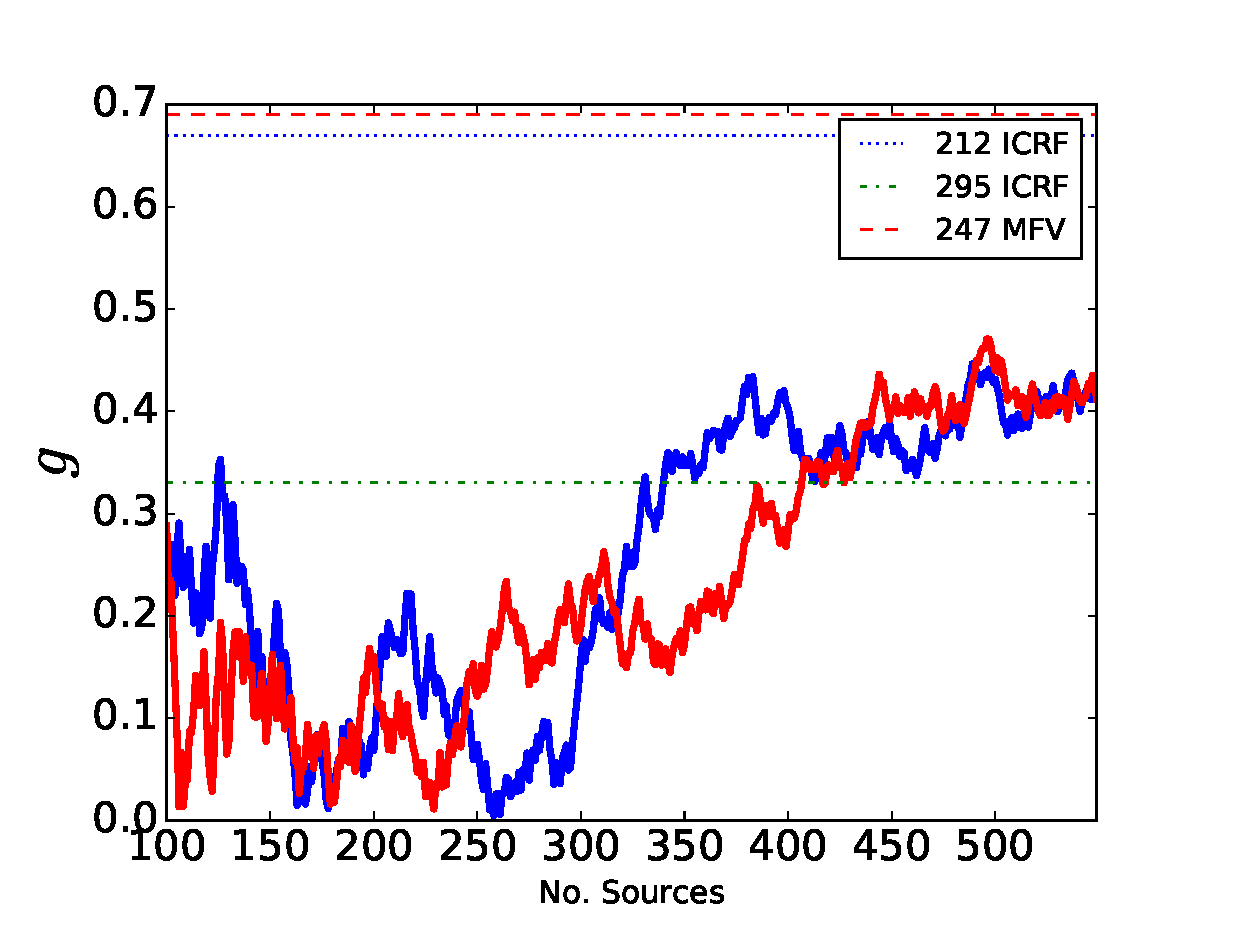
\includegraphics[width=\hsize]{figures/Simulation.eps}
      \caption{
      The results of simulation. The blue and red line are corresponding result of rank1 and rank2 respectively.
              }
         \label{Fig:sim}
   \end{figure}

\subsection{Consideration on above two respects}
The results in the above sections show that it is necessary to balance the consideration on axial ability and sky distribution. A simple way is to average $r$ and $\omega$, as shown in Fig. \ref{Fig:com_num}. More sources usually means a good sky coverage while smaller $(r+\omega)/2$ means good behaviors in axial stability and uniform distribution. Balancing these two factors, four sets of sources are selected to be defining sources, as indicated in in Fig. \ref{Fig:com_num} by red and blue points. For rank1, the numbers of sources are 307 and 366, referred as "Sou307" and "Sou366". And the numbers are 304 and 324 for rank2, similarly referred as "Sou304" and "Sou324". The linear drift of sources in these four sets are shown in Fig. \ref{Fig:Liner_drift_4}, most sources showing a tiny linear drift. And the corresponding statical information is given in Table.  \ref{Tab:Mean_Dec}, Table.\ref{Tab:Axi} and Table.\ref{Tab:Sim}.

	\begin{table}
	\caption{Mean declination and Source}
	\label{Tab:Mean_Dec}
	\centering
	\begin{tabular}{ccc}
	\hline\hline
Source &Mean           &Number of         \\
Set    &declination    &ICRF2 defining    \\
Sou307& 9.41$^{\circ}$ &                 \\
Sou366& 6.48$^{\circ}$ &                 \\
Sou304& 0.68$^{\circ}$ &                 \\
Sou324& 0.54$^{\circ}$ &                 \\
\hline
	\end{tabular}
	\tablefoot{The mean declination for 212 ICRF, 295 ICRF2 and 247 MFV are 4.80$^{\circ}$, 0.70$^{\circ}$, and 16.89$^{\circ}$ respectively.}
	\end{table}
	
	\begin{table}
	\centering
	\caption{Axial stability}
	\label{Tab:Axi}	
	\begin{tabular}{ccccc}
\hline\hline
Source &               &               &               &       \\
Set    &$r_1$          &$r_2$          &$r_3$          &$r$    \\
Sou307 &0.63$\pm$0.16 &-0.05$\pm$0.17 &4.35$\pm$0.12 &4.40$\pm$0.26 \\
Sou366 &0.99$\pm$0.15 &-3.40$\pm$0.16 &4.90$\pm$0.11 &6.04$\pm$0.24 \\
Sou304 &1.37$\pm$0.15 &-2.41$\pm$0.16 &4.35$\pm$0.12 &5.16$\pm$0.25 \\
Sou324 &1.70$\pm$0.15 &-3.41$\pm$0.16 &4.64$\pm$0.11 &6.01$\pm$0.25 \\
\hline
	\end{tabular}
	\tablefoot{The units: $\mu as \cdot yr^{-1} $.}
	\end{table}	
	
	\begin{table}
	\caption{Sky distribution simulation}
	\label{Tab:Sim}
	\centering
	\begin{tabular}{ccccc}
\hline\hline
Source &               &               &               &\\
Set    &$\omega_1$     &$\omega_2$     &$\omega_3$     &$\omega$  \\
Sou307 &0.07$\pm$0.07 & 0.18$\pm$0.07 & 0.00$\pm$0.07 &0.19$\pm$0.12 \\
Sou366 &0.21$\pm$0.07 & 0.13$\pm$0.06 &-0.01$\pm$0.06 &0.24$\pm$0.11 \\
Sou304 &0.16$\pm$0.07 &-0.03$\pm$0.07 &-0.00$\pm$0.07 &0.16$\pm$0.12 \\
Sou324 &0.16$\pm$0.01 & 0.01$\pm$0.07 &-0.00$\pm$0.07 &0.16$\pm$0.12 \\
\hline
	\end{tabular}
	\tablefoot{The units: $\mu as \cdot yr^{-1} $.}
	\end{table}

	\begin{figure}
   \centering
   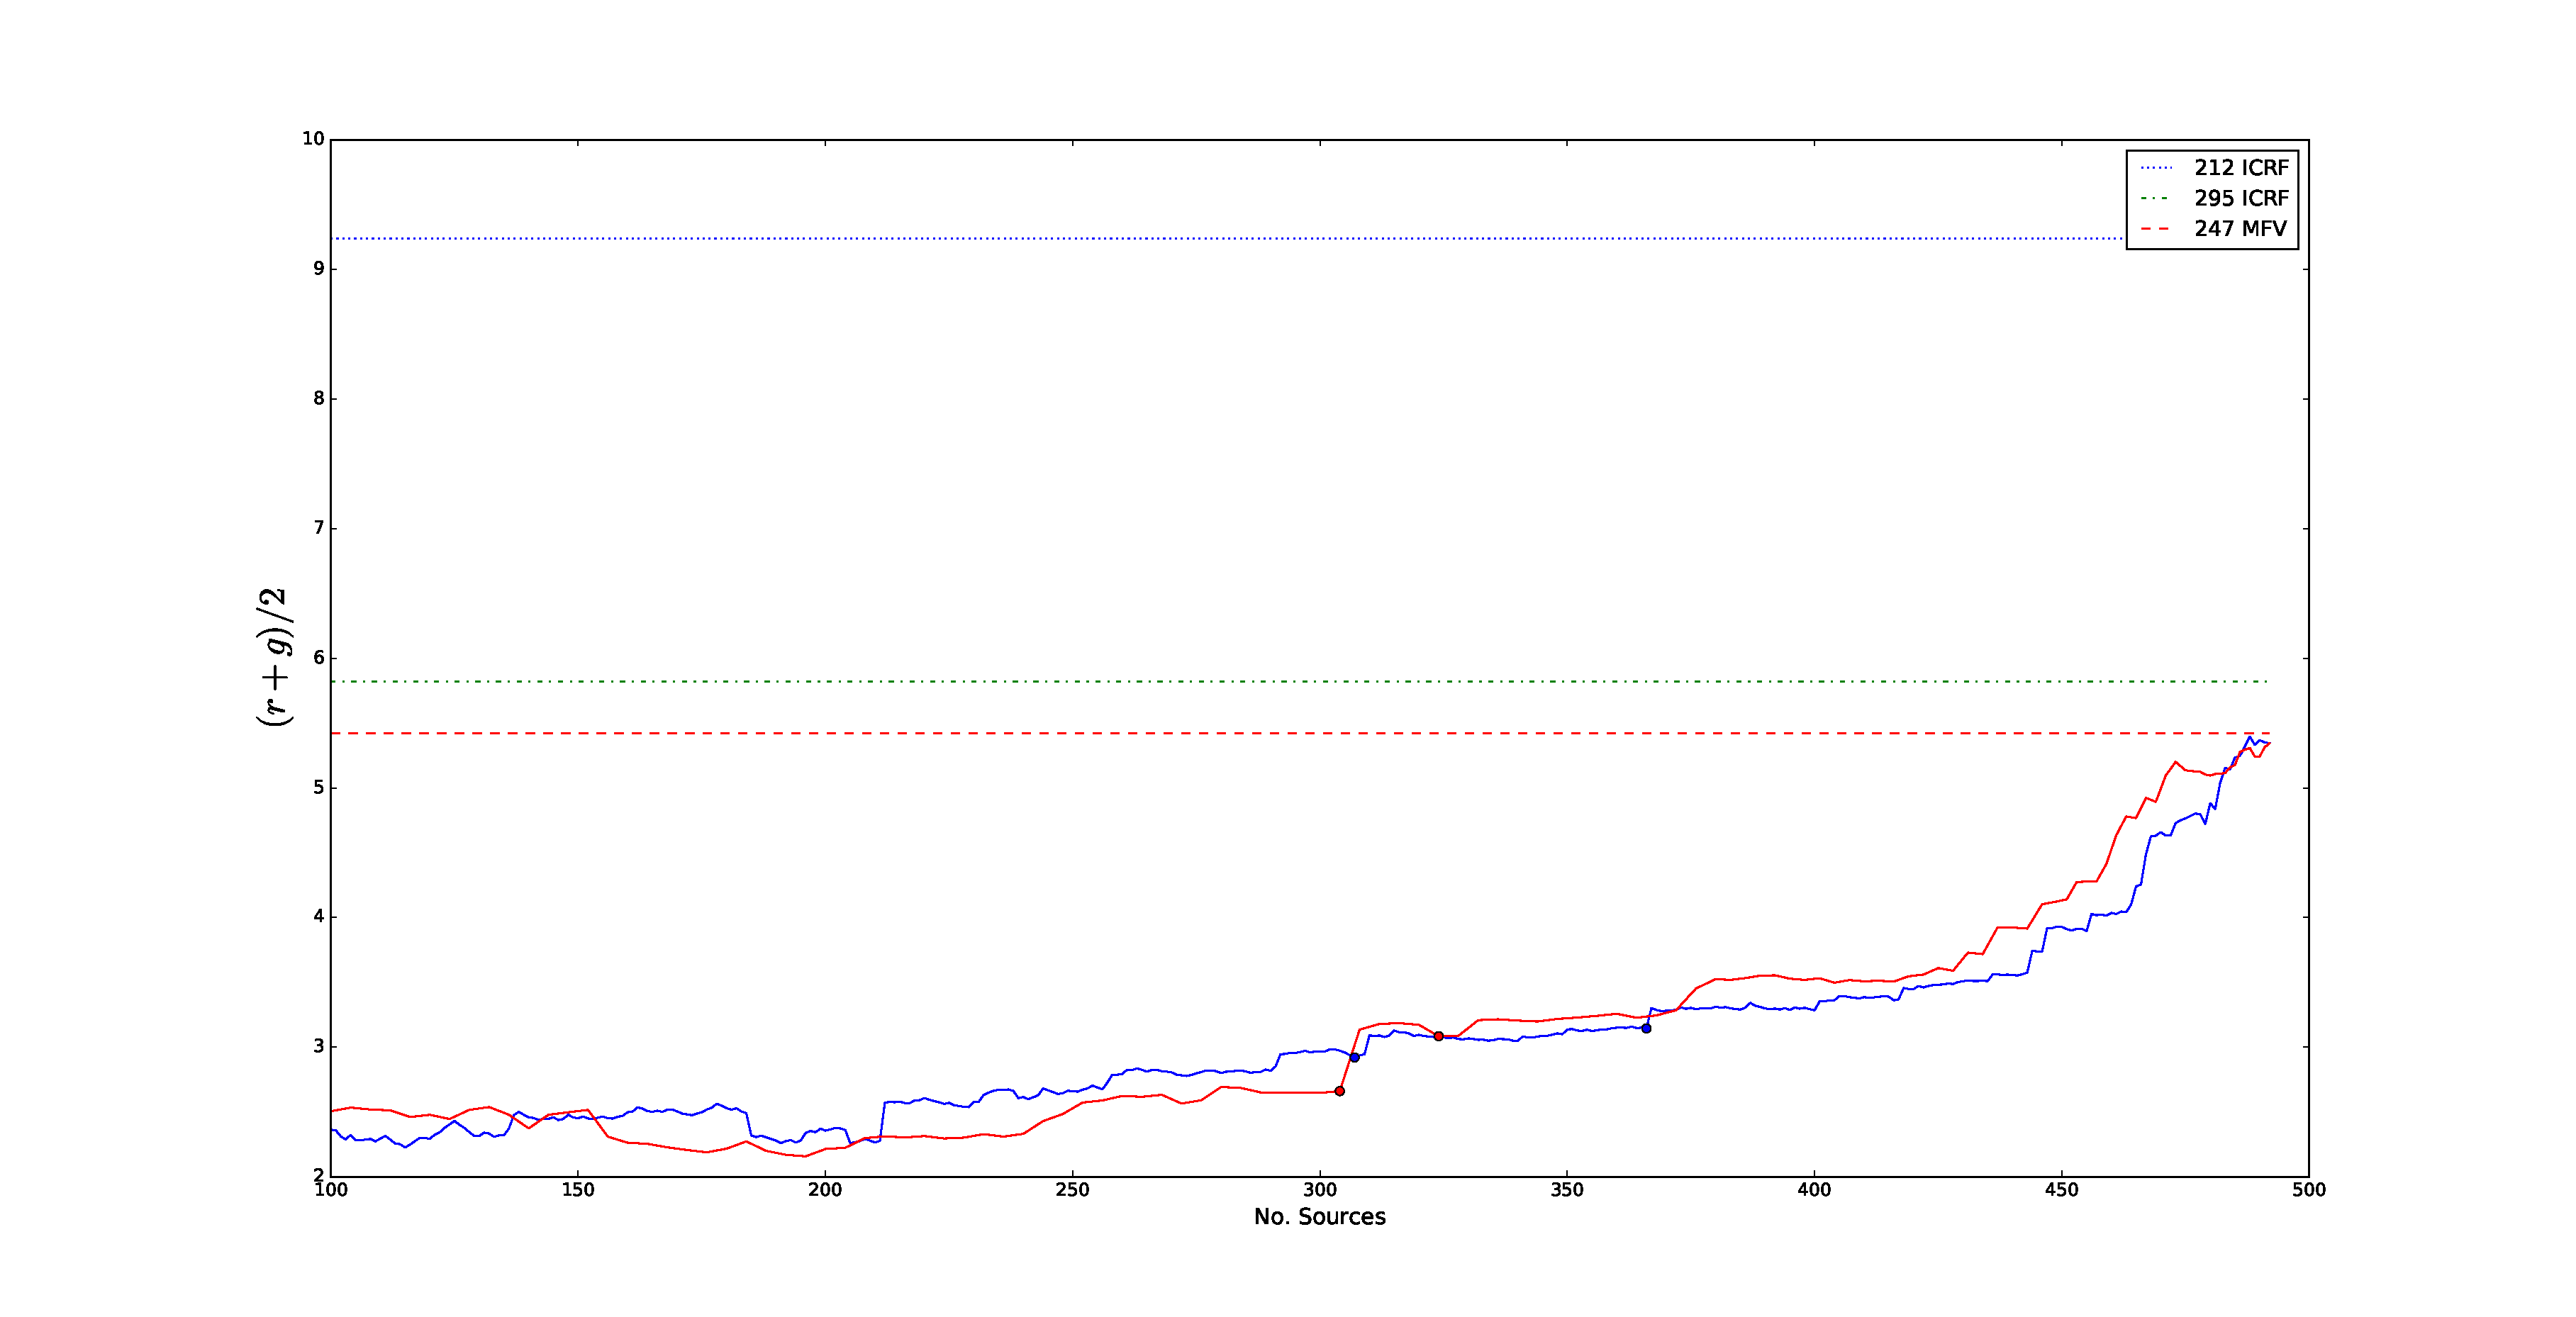
\includegraphics[width=\hsize]{figures/Combination.eps}
      \caption{
      The results of simulation. The blue and red line are corresponding result of rank1 and rank2 respectively. The red and blue points represent 4 sets of sources to be considered as defining sources.
              }
         \label{Fig:com_num}
   \end{figure}
   
   \begin{figure*}
   \centering
   \subfigure[Sou307]{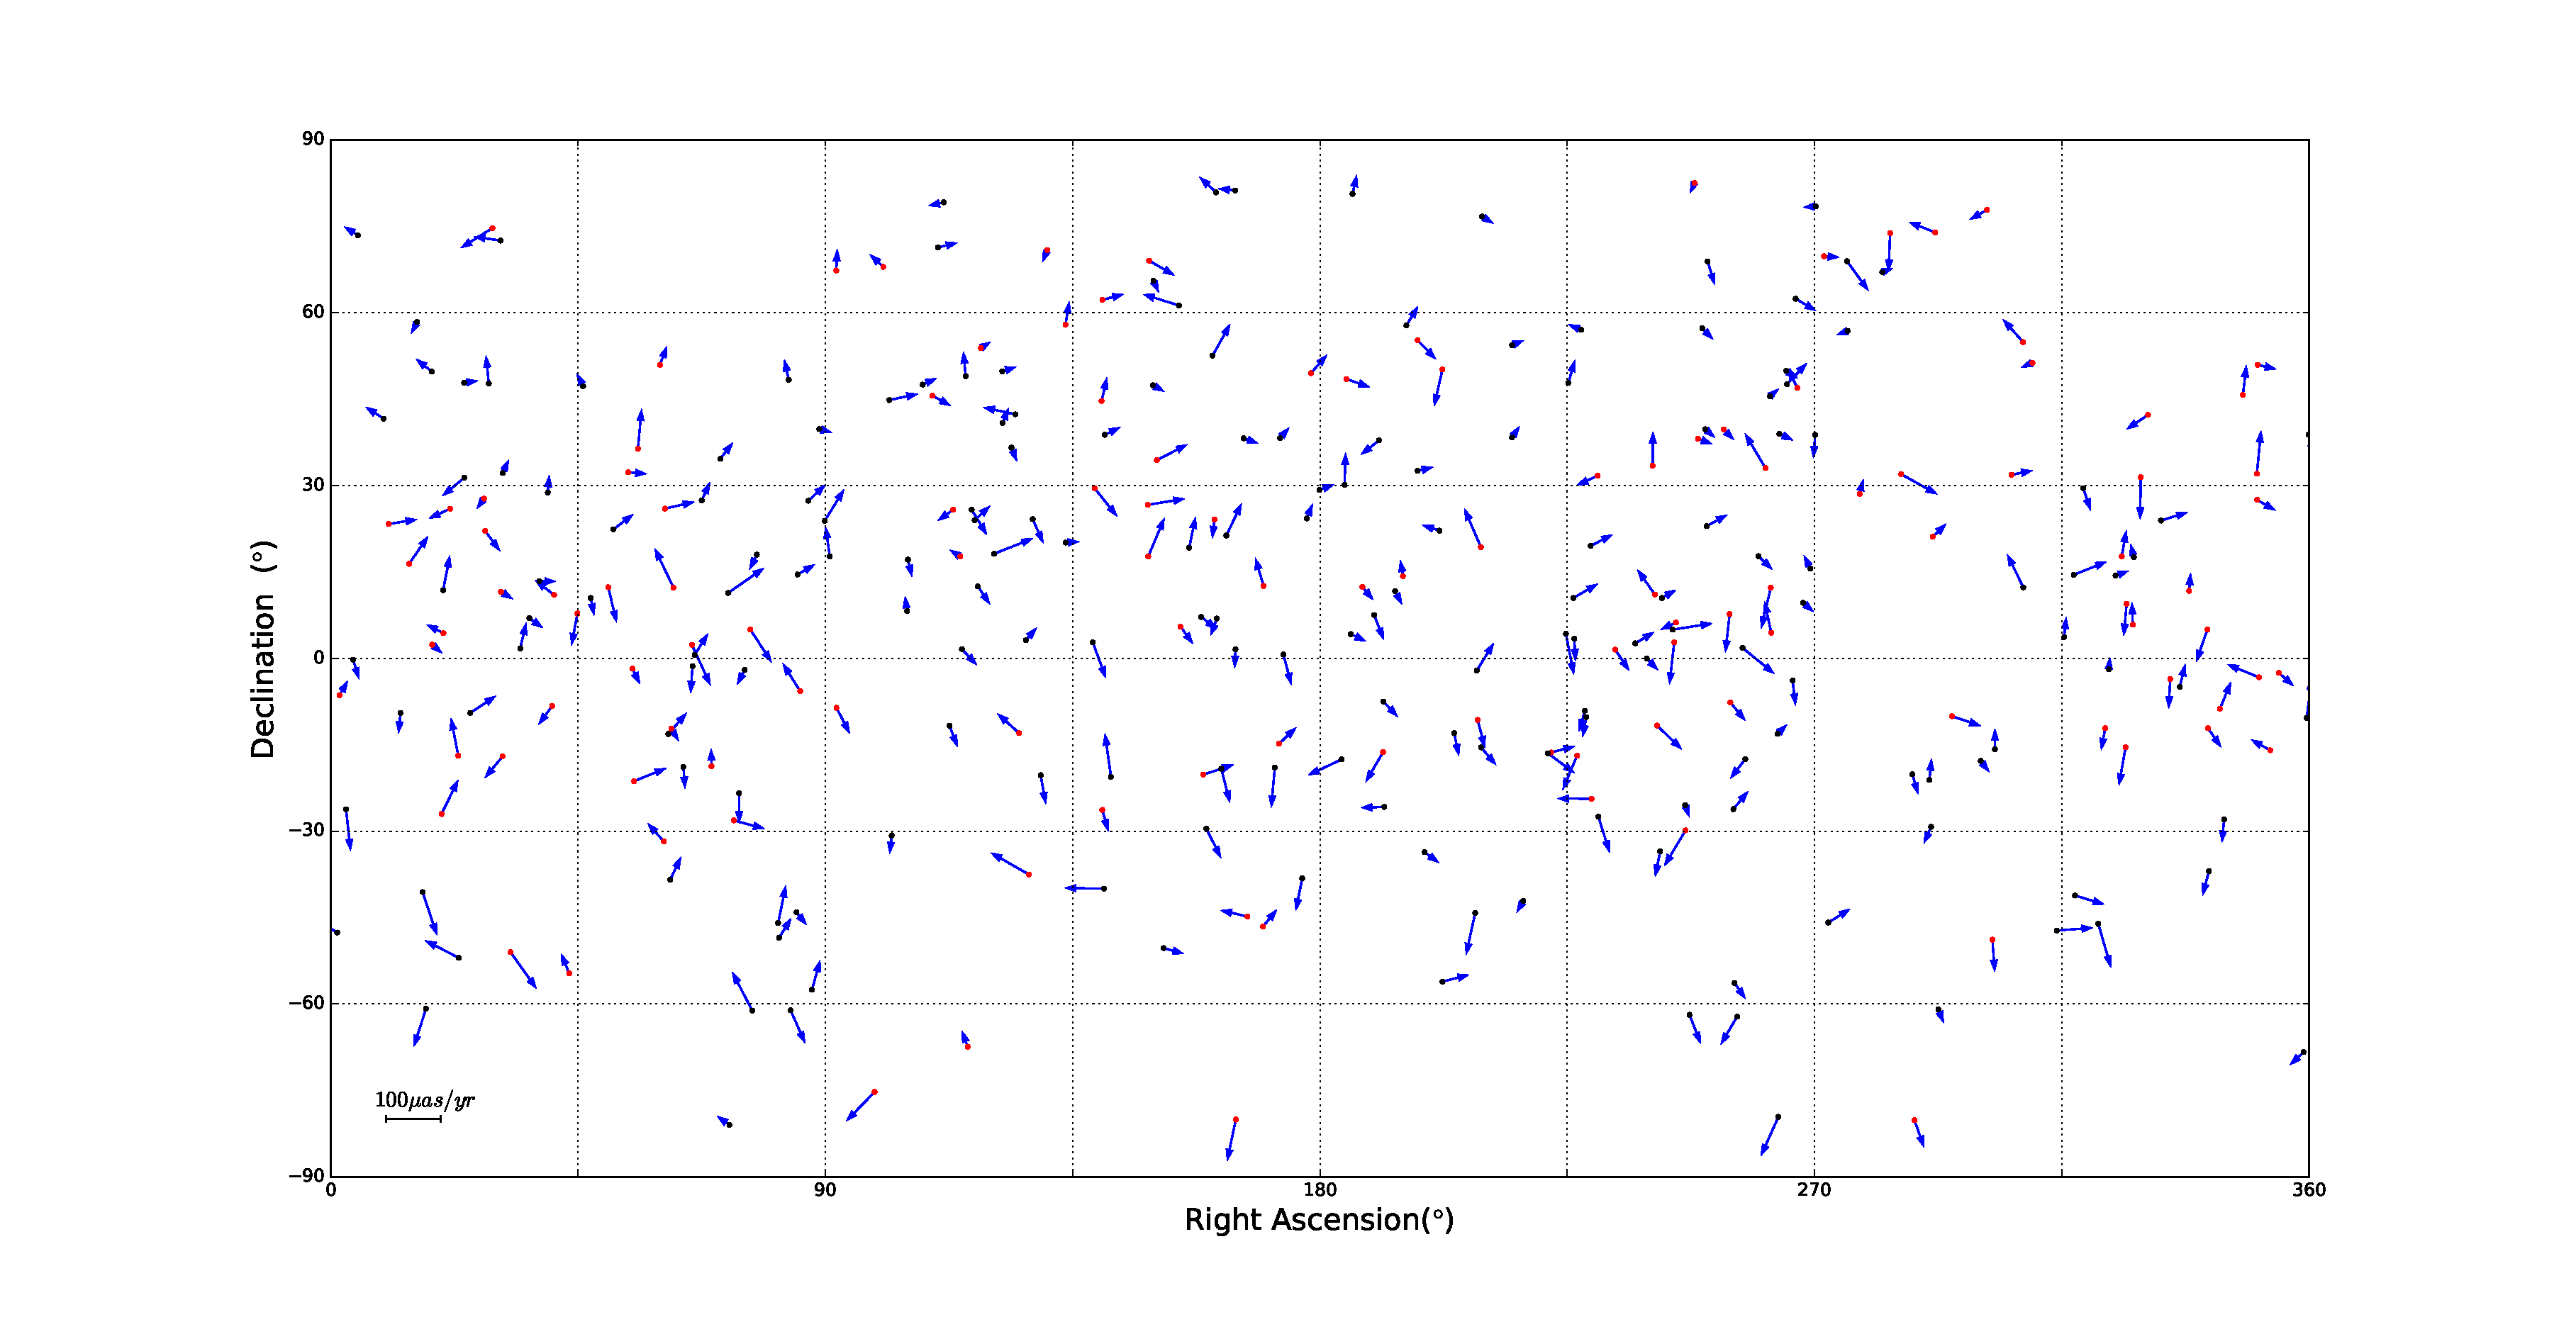
\includegraphics[width=0.5\hsize]{figures/Linear_drift_307r1.eps}}
   \subfigure[Sou366]{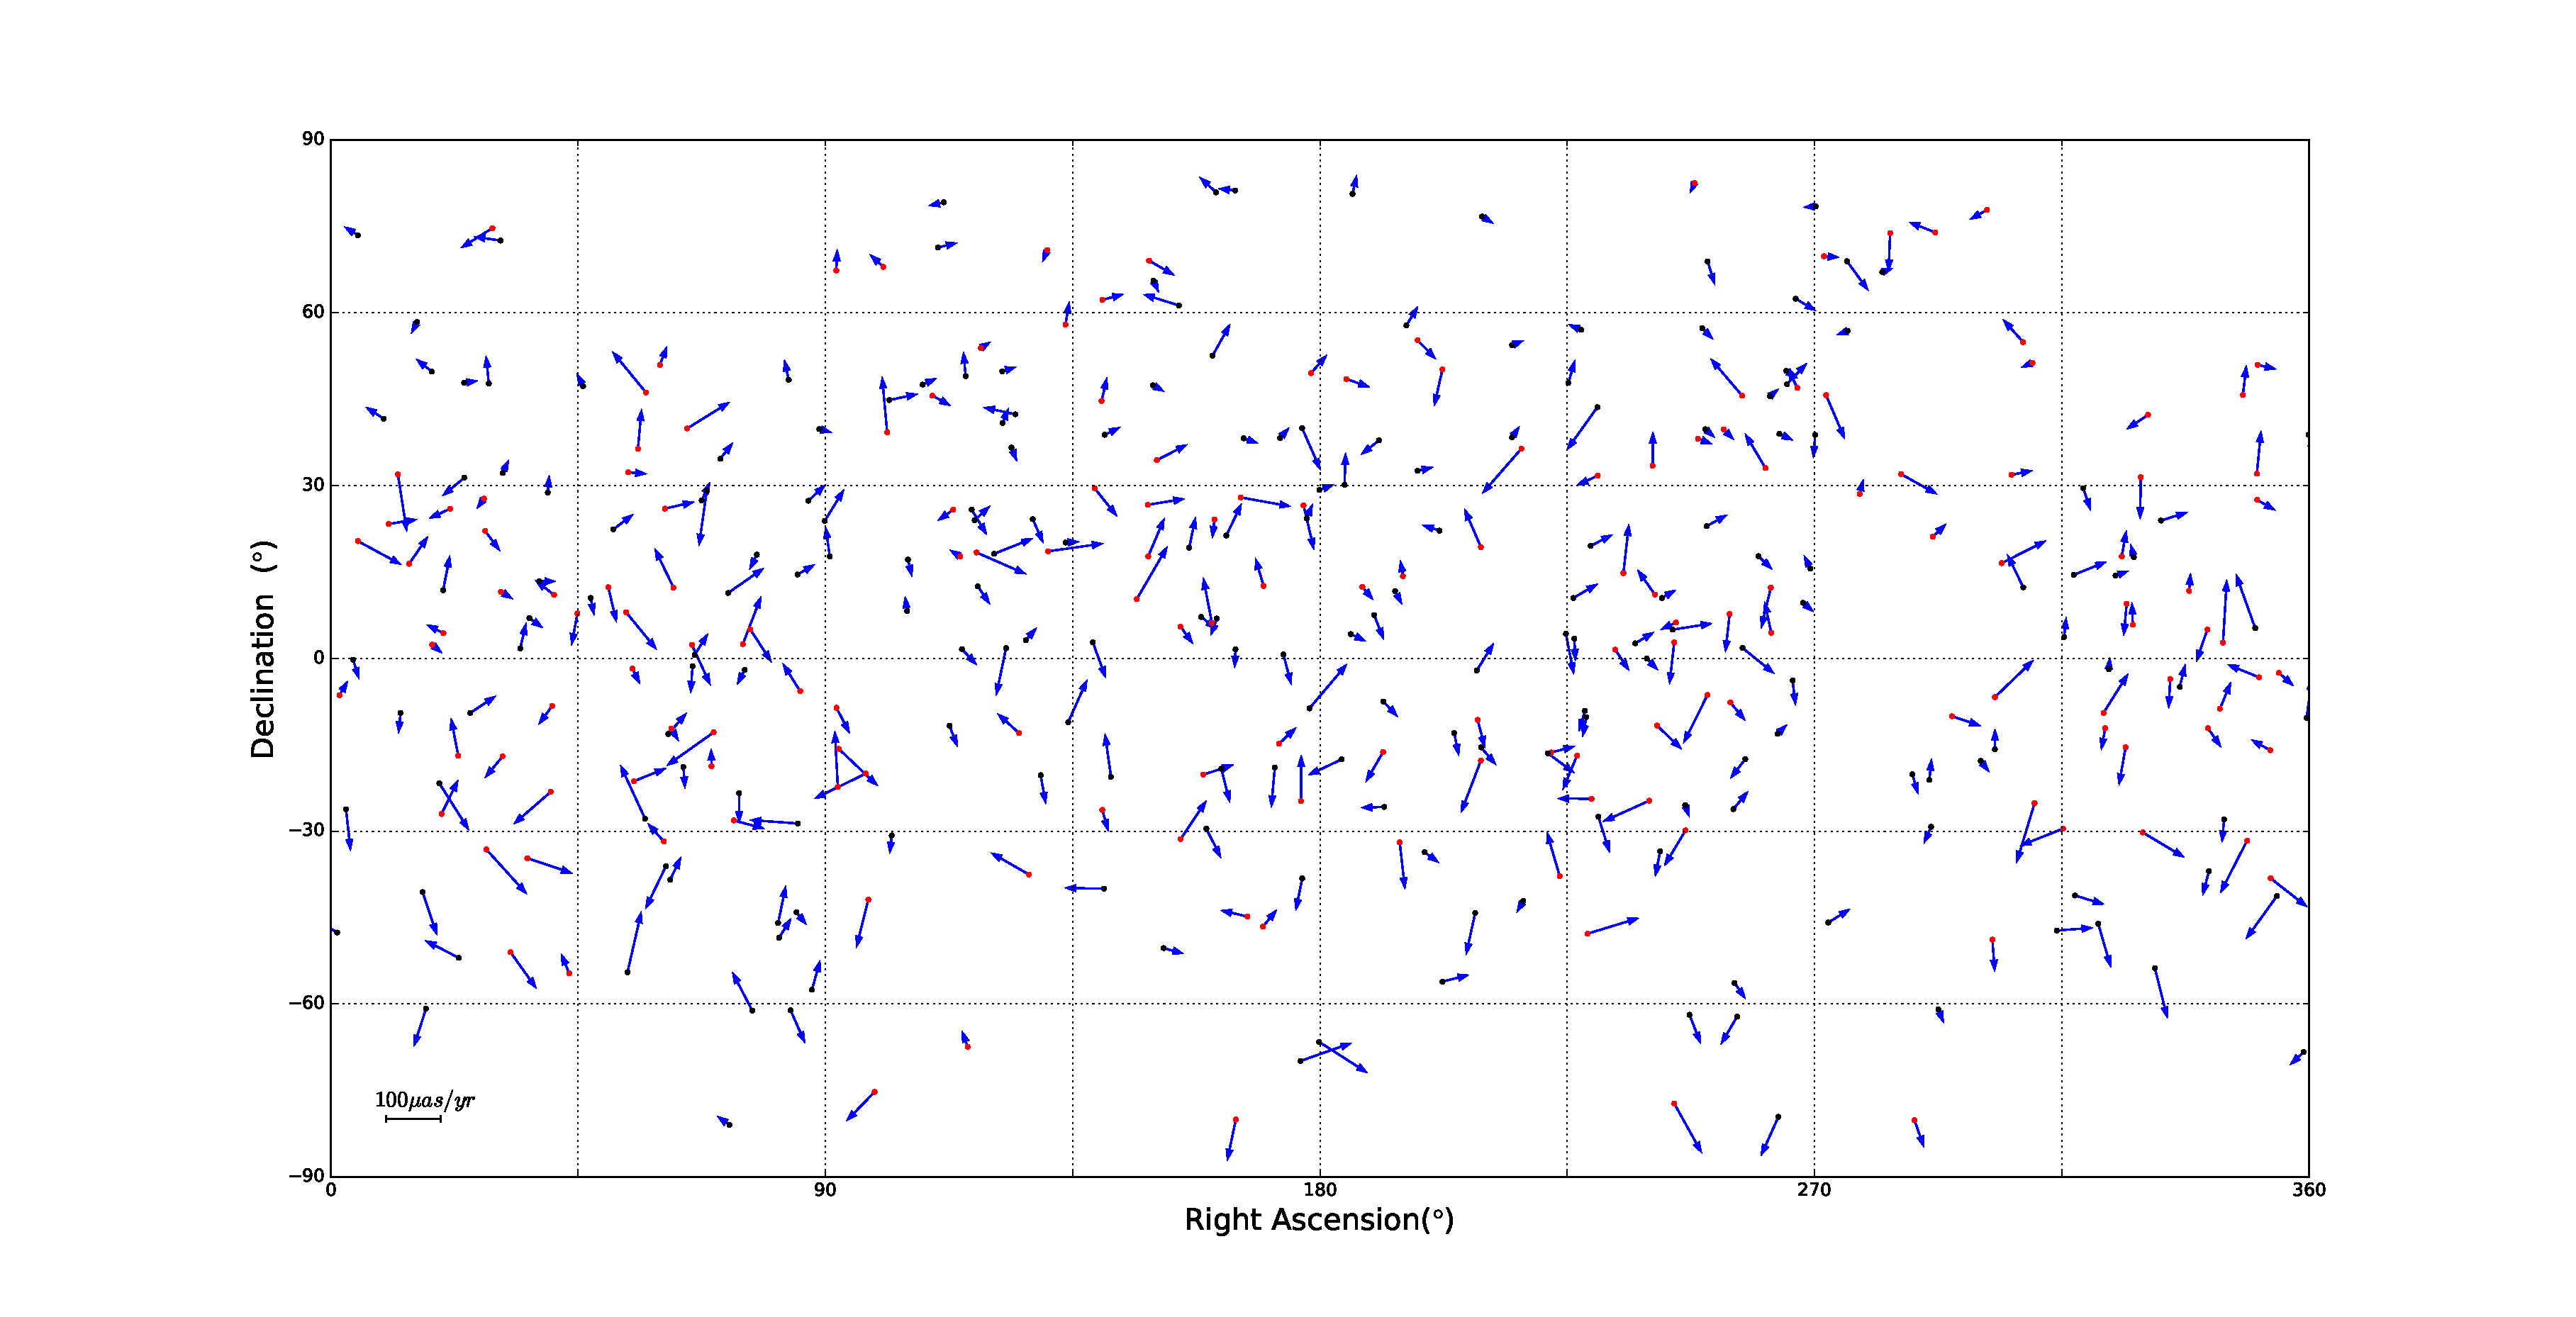
\includegraphics[width=0.5\hsize]{figures/Linear_drift_366r1.eps}}
   \subfigure[Sou304]{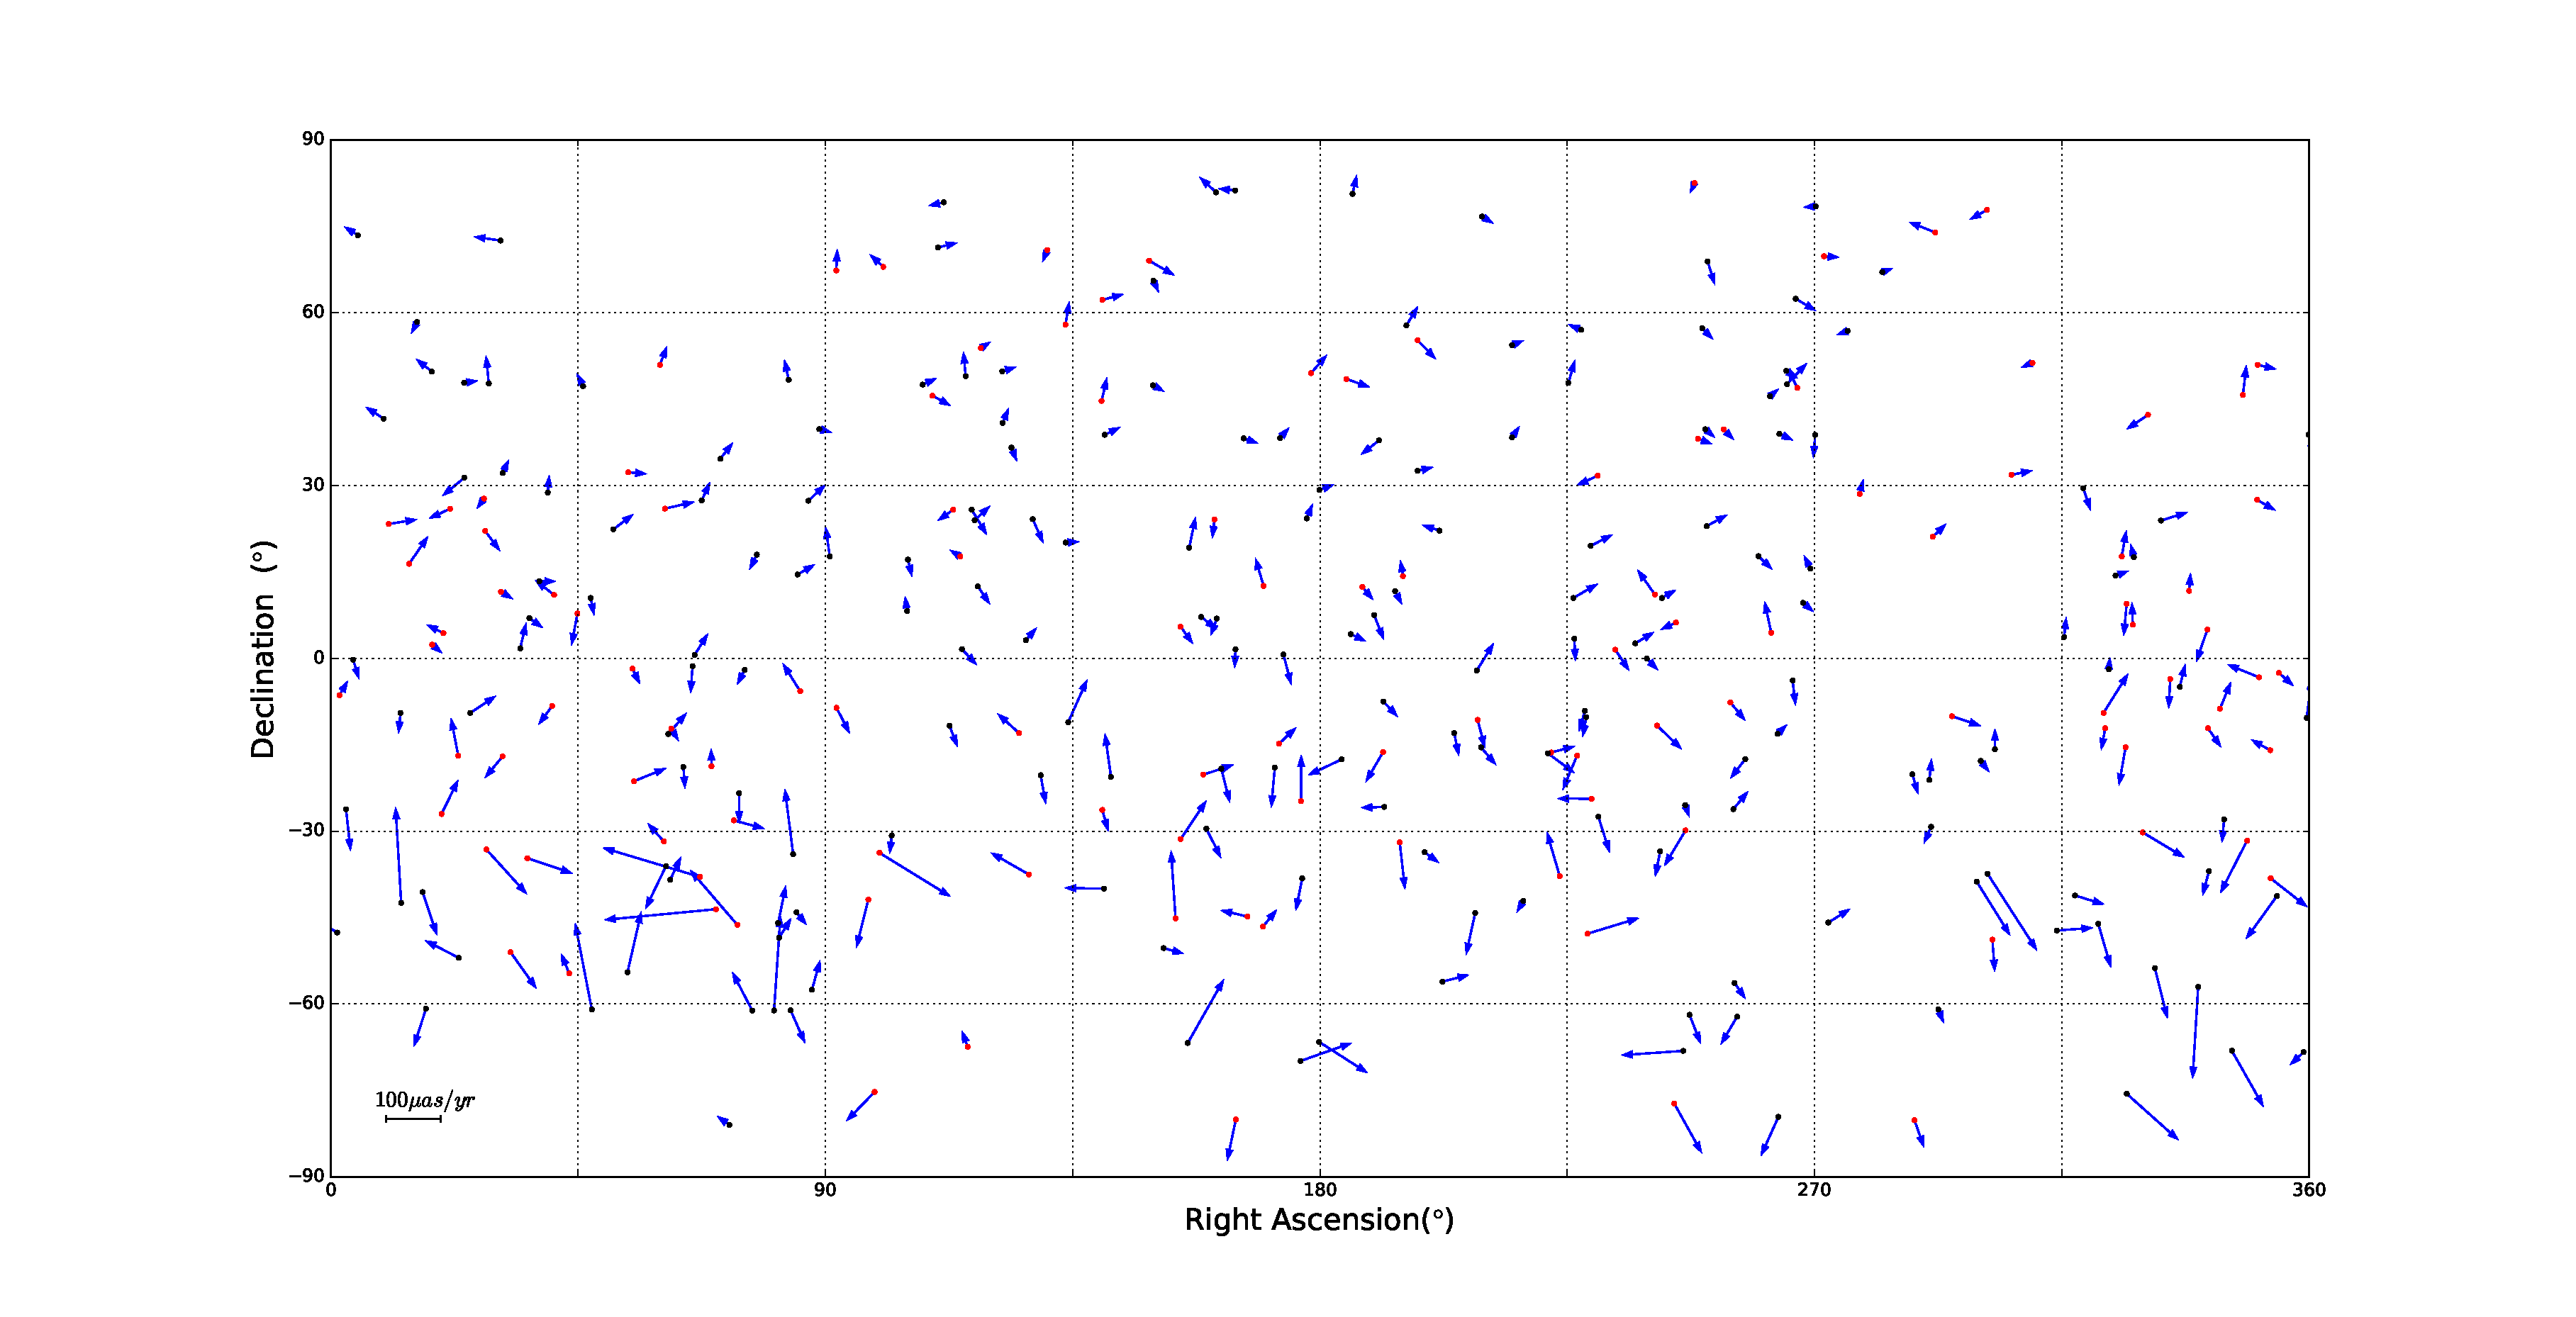
\includegraphics[width=0.5\hsize]{figures/Linear_drift_304r2.eps}}
   \subfigure[Sou324]{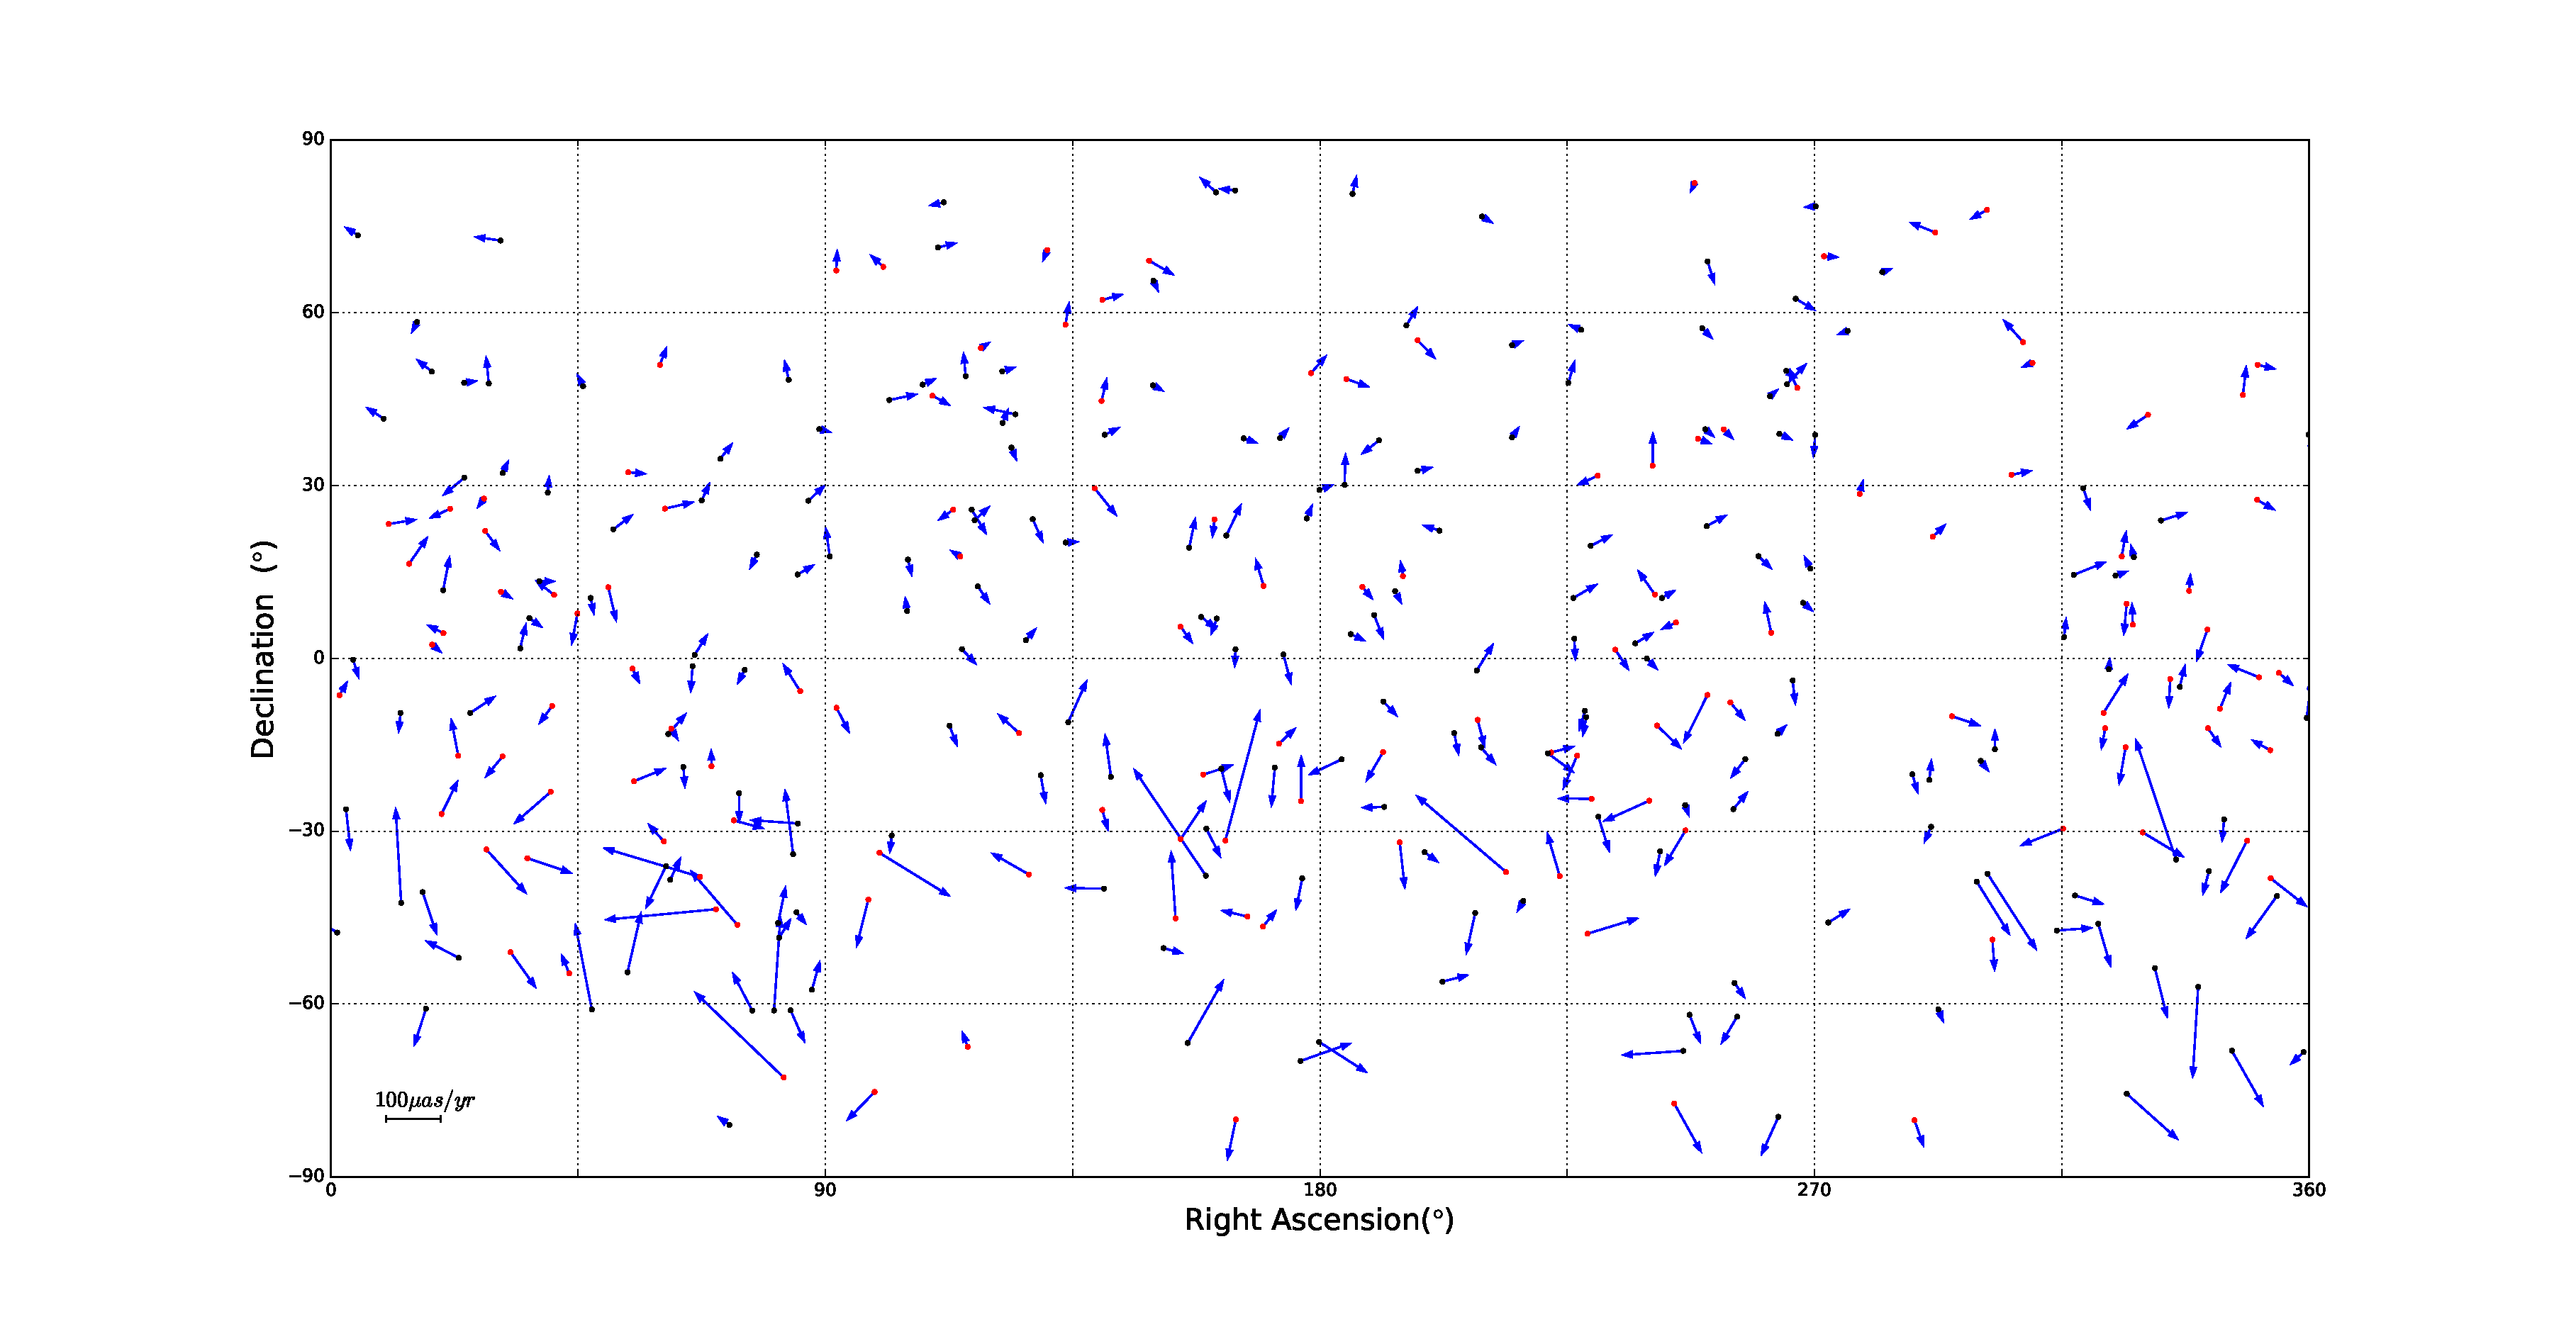
\includegraphics[width=0.5\hsize]{figures/Linear_drift_324r2.eps}}
      \caption{
      Linear drift of 4 sets of sources to be considered as defining sources. The red points means that the sources is included in 295 ICRF2 defining sources.
              }
         \label{Fig:Liner_drift_4}
   \end{figure*}
%-----------------------------------------------------------------
\section{Conclusions}\label{sect:conclusion}
With the time series of coordinates over 30 years for sources, some of ICRF2 defining appear to be unstable and not suitable to defining a celestial frame. 4 sets of sources with improved in both axial stability and uniform sky distribution are recommended.
%-----------------------------------------------------------------

\begin{acknowledgements}
      
\end{acknowledgements}

\bibliographystyle{aa}
%\bibliography{bibtex/aa.bib}
\bibliography{bibtex/SourcesSelection}
\end{document}
